\documentclass{beamer}
\usetheme{CambridgeUS}
\usefonttheme{serif}
\setbeamertemplate{navigation symbols}{}

\usepackage{ctex}
\usepackage{amsmath,amssymb,amsfonts,bm}
\usepackage{graphicx,subfigure}
\usepackage{adjustbox}
\usepackage{color,xcolor}
\usepackage{tikz}

% 自定义数学公式
\newcommand{\abs}[1]{\left\vert#1\right\vert}
\newcommand{\floor}[1]{\left\lfloor{#1}\right\rfloor}
\newcommand{\ceil}[1]{\left\lceil{#1}\right\rceil}
\newcommand{\sbrace}[1]{\left(#1\right)}
\newcommand{\mbrace}[1]{\left[#1\right]}
\newcommand{\bbrace}[1]{\left\{#1\right\}}
\newcommand{\eval}[2]{\left.{#1}\right|_{#2}}
\newcommand{\conj}[1]{{\rm conj}\sbrace{#1}}
\newcommand{\ALLP}{\mathcal{A}}
\newcommand{\PS}{\mathcal{P}}
\newcommand{\dd}[1]{\mathrm{d}#1}
\newcommand{\ii}[1]{\int\!{#1\dd x}}
\newcommand{\VecNorm}[1]{\left\Vert#1\right\Vert}% 向量模
\newcommand{\spell}[1]{#1}
\newcommand{\up}[1]{^{(#1)}}
\newcommand{\TT}{^\top}% 矩阵转置
\newcommand{\OO}{\ensuremath{\mathbb O}}% n 阶展开多项式余项
\newcommand{\OC}{\ensuremath{\mathcal O}}% 算法复杂度
\newcommand{\lfrac}[2]{#1/#2}
\newcommand{\DIF}[1]{\ensuremath{\frac{\partial}{\partial #1}}}
\newcommand{\DIFF}[2]{\ensuremath{\frac{\partial #1}{\partial #2}}}
\newcommand{\cd}[1]{\,\texttt{#1}\,}
\newcommand{\dbrace}[1]{
  \Bigl\{
    #1
  \Bigr\} 
}
\newcommand{\red}[1]{{\color{red}#1}}

\usepackage{textcomp}
\newcommand{\tpa}{\checkmark}
\newcommand{\tpb}{$-$}
\newcommand{\tpc}{\texttimes}

\newcommand{\Painleve}{Painlev{\'e}}

\title[]{非线性微分方程解析求解与可积性分析的机械化算法研究}
\author[]{李志斌, 柳银萍, 余江涛\\[1em] 华东师范大学}
\date{\today}

\begin{document}
\frame{
    \tikz[overlay,remember picture]\node[opacity=0.1]at (current page.center){
\includegraphics[width=0.7\paperheight]{../paper/sty/ecnu_logo.pdf}};
    \titlepage
}

\begin{frame}
     数学问题要机械化,首先要代数化,进而机械化。
\end{frame}
\begin{frame}{内容}
\begin{itemize}
  \item 前期工作回顾; 
  \item 近期进一步的创新工作. 
  \end{itemize}
\end{frame}
\begin{frame}{前期工作回顾}
  非线性微分方程精确解的构造算法与可积性分析算法研究。
  \begin{itemize}
    \item 齐次平衡方法与齐次平衡原则\\[1mm]
    \item 直接代数方法(子方程方法,函数展开法)\\[1mm]
    \item Painlev\'e 测试与Painlev\'e截断展开法 \\[1mm]
    \item Hirota 双线性方法 \\[1mm]
    \item 对称方法 \\[1mm]
    \item B\"acklund 变换与Darboux 变换\\[1mm]
    \item 无穷守恒律构造算法 
  \end{itemize}
\end{frame}
\begin{frame}{齐次平衡方法与齐次平衡原则}
  齐次平衡方法是构造非线性演化方程精确解的一种普适性方法,该方法是1993年我和王明亮等人提出的。齐次平衡方法是根据方程最高阶部分可部分平衡的原则, 确定方程的解应具有的一般形式, 再将这种形式代回原方程进行求解. 
  例如burgers方程
  \[
    u_t+2uu_x-pu_{xx}=0,
  \]
 假设$u=f^{(m+n)}(\phi){\phi_x}^m{\phi_t}^n+\cdots+f(\phi)$关于$x$和$t$的低于$m+n$阶偏导数的适当的线性组合,$\phi(x,t)$称为方程的拟解. 则有
 \[
   u_{xx}= f^{(m+n+2)}{\phi_x}^{m+2}{\phi_t}^n+\cdots     
\]
  \[
uu_x=f^{(m+n)}\cdot f^{(m+n+1)}{\phi_x}^{m+1}{\phi_t}^n +\cdots  
\]
上两式最高阶部分平衡:$m+2=2m+1,\,\, n=2n$, 故 $m=1,n=0$.
\end{frame}
\begin{frame}
则上述假设式简化为:
\begin{equation}\label{u_f}
  u=f\,'(\phi){\phi_x},
\end{equation}
将其代入原方程得
\begin{equation}\label{eq1}
  \begin{array}{ll}
 u_t+2uu_x-pu_{xx}=(2f^{\,'}f^{\,''}-pf^{\,'''}) {\phi_x}^3+f^{\,''}(\phi_x\phi_t-3p\phi_x\phi_{xx}+2{\phi_x}^2)\\[2mm]+2{f^{\,'}}^2\phi_x\phi_t+f^{\,'}(\phi_{xt}-p\phi_{3x}).
  \end{array}
\end{equation}
先让${\phi_x}^3$的系数为零,得$f(\phi)$的ODE
\[
  2f^{\,'}f^{\,''}-pf^{\,'''} =0,
\]
该方程有一个解:
\begin{equation}\label{sol1}
 f=-p\ln\phi, 
\end{equation}
且有 
\[
 {f^{\,'}}^2=pf^{\,''},
\]
\end{frame}
\begin{frame}
将上两式代入方程(\ref{eq1}),化简得到
\begin{equation}\label{eq2}
u_t+2uu_x-pu_{xx}=(f^{\,'}\phi_x+f^{\,'}\frac{\partial}{\partial x})(\phi_t-p\phi_{xx}),
\end{equation}
故只要满足热传导方程
\begin{equation}\label{eq4}
  \phi_t-p\phi_{xx}=0,
\end{equation}
  则方程(\ref{eq2})的左边为零。将(\ref{sol1})代入(\ref{u_f}),就得到所谓的Core-Hopf变换
\[
  u=-p\dfrac{\phi_x}{\phi}.
\]
由于方程(\ref{eq4})是线性方程,由线性叠加原理,可构造出其各种形式的精确解,将这些解代入Core-Hopf变换,即可获得Burgers方程各种类型的解。特别地,当假设
\[
  \phi(x,t)=1+e^{kx+ct} ,
\]
则可得到原方程的孤波解
\[
  u \left( x,t \right) =-1/2\,pk-pk\tanh \left( {k}^{2}pt+kx \right).
\]
\end{frame}
\begin{frame}
从这个实例可以看出,基于齐次平衡方法可获得很好的副产品:
   \begin{itemize}
    \item 确定解的阶数的思路即为齐次平衡原则,很多直接代数方法都是基于该原则发展起来的,Painlev\'{e}测试算法也应用了齐次平衡原则;
    \item 由齐次平衡方法可获得很丰富的变换,如上例中的Core-Hopf变换;
    \item 当假设拟函数$\phi(x,t)=1+e^{kx+ct}$时,所获得的解往往可表示为tanh函数的有限级数。基于此,双曲正切方法应运而生。 
   \end{itemize}
\end{frame}
\begin{frame}{直接代数方法}
直接代数方法,通常也被称为子方程方法,或函数展开法。如双曲正切方法、椭圆函数展开法、形变映射方法等。这些方法的思路都是用低阶方程的解来构造高阶方程的解。
如双曲正切方法就是将所求的解假设为双曲正切函数的有限级数,因为双曲正切函数是如下Riccati方程的解:
\[
   T\,'=R(1-T^2).  
\]
从该方程可以看出,将解的假设式代入原方程可得到$T$函数的多项式方程,令其不同次幂项的系数为零,得到一个非线性代数方程组。需要指出,在这类子方程方法中,所获得的非线性代数方程组的求解是一个计算瓶颈。吴消元法的提出,为非线性代数方程组的求解提供了一个强有力的工具。
我较早地接触到了吴消元法,并将该方法应用到双曲正切方法中,将该方法系统化,进而完全算法化和机械化。
\end{frame}
\begin{frame}
  在该方法的基础上,相继诞生了一系列子方程方法. 如: 
  
  耦合的Riccati方程
  \[
    f(\xi)\,'=Rg(\xi)^2,\,\,g(\xi)\,'=\mu f(\xi) g(\xi),
  \]
  具有解$f=tanh(\xi),\,\,g=sech(\xi)$. 
 
  三耦合的Riccati方程
  \[
    f(\xi)\,'=g(\xi)h(\xi),\,\,g\,=-fh,\,\,h\,'=-m^2fg,\,\, 0\leq m \leq 1.
  \]
  具有解$f=sn(\xi,m),\,\,g=cn(\xi,m),\,\,h=dn(\xi,m).$
  
  椭圆方程
  \[
      {f\,'}^2=c_0+c_1 f +c_2 f^{\,2}+c_3f^{\,3}+c_4f^{\,4},  
  \]
  根据$c_i(0 \le i \le 4)$的不同取值,该方程具有一系列解,包括多项式解、有理函数解、指数函数解、双曲函数解、Jacobi椭圆函数解等。
\end{frame}
\begin{frame}{Painlev\'e 测试算法}
Painlev\'e 测试算法是判断一个非线性微分方程是否可积的必要条件。但是基于P测试算法,也可获得很好的副产品,如:
\begin{itemize}
\item 基于P截断展开可获得Hirota双线性方法中所需要的变换;
\item 基于截断展开可构造非线性演化方程的精确行波解; 
\item 基于P测试算法可进一步获得原方程的可能的Lax对等。
\end{itemize} 
我和学生研究了Painlev\'e 测试的机械化算法,并研发了相应的自动推导软件wkptest,该软件不仅可自动检测输入方程是否通过P测试,还可给出Painlev\'e 截断展开式,该展开式即为Hirota双线性方法中所需的变换。基于该截断展开式可计算精确解等。该软件对变系数微分方程或方程组也有效。
       
\end{frame}

\begin{frame}{Hirota方法与简单Hirota方法}
Hirota方法是构造非线性演化方程孤子解的有效方法,但是应用Hirota方法构造孤子解时,首先要将方程转化为双线性形式,然而只有可积方程只有双线性形式。简单Hirota方法绕过了双线性形式,因此,应用简单Hirota方法也可构造不可积方程的孤子解。我们小组完全实现了简单Hirota方法,可自动推导非线性演化方程的孤子解。需要说明,n-孤子解的公式对可积方程有效,往往对不可积方程不成立。

近期我们小组给出了不可积方程n-孤子解公式成立的一种约束条件。并基于孤子解,进一步计算方程的呼吸子等周期波解、Lump解等。我们小组也实现了相应的算法,所研发的软件TwSolver可自动推导出非线性演化方程的孤子解及可能的breather解,Lump解等。

需要说明,软件TwSolver中所需的变换即有Painlev\'e 测试软件给出。\\[2mm]

\mbox{}\hskip 3cm 软件演示
  
\end{frame}
\begin{frame}{达布变换}
  达布变换与贝克隆变换也是构造非线性微分方程精确解的有效方法。我和学生在达布变换和贝克隆变换的构造算法和自动推理方面也做过一些工作。达布变换的文章列表如下:
\begin{itemize}
  \item[1.] Qilao Zha, Zhibin Li. Darboux transformation and multi-solitons for complex mKdV equation. Chinese Physics Letters, 2008, 25(1): 8.
  \item[2.]	Qilao Zha, Zhibin Li. Darboux transformation and various solutions for a nonlinear evolution equation in (3+ 1)-dimensions. Modern Physics Letters B, 2008, 22(30): 2945-2966.
  \item[3.]	Qilao Zha, Zhibin Li. Periodic wave solutions of generalized derivative nonlinear Schrödinger equation. Chinese Physics Letters, 2008, 25(11): 3844.
  \item[4.]	Qilao Zha, Zhibin Li. Solitary wave solutions to the generalized coupled mKdV equation with multi-component. Journal of Mathematical Analysis and Applications, 2009, 359(2): 794-800.
\end{itemize}
\end{frame}
\begin{frame}{自贝克隆变换的机械化算法}
很多具有如下形式的非线性演化方程
\begin{equation}\label{eq344}
E(u,\,u_t,\,u_x,\,u_{xx},\,\cdots)=0,
\end{equation}
都具有自 B\"{a}cklund\,变换
\begin{equation}\label{eq345}
(u\,+ a\,v)_t = H,\hskip 0.5cm (c\,u\, + v)_x =P(u + a\,v),
\end{equation}
其中 $a,\,c$\,是常量, $H$\,是$u,\,v$\,及其偏导数的函数.

例如, KdV\,方程
\begin{equation}\label{KdV}
w_t+6\,w\,w_x+w_{xxx}=0,
\end{equation}
通过变换 $w=u_x$, 我们得到
\begin{equation}\label{KdVeq2}
u_{xt}+(3(u_x)^2+u_{xxx})_x=0.
\end{equation}
方程(\ref{KdVeq2}) 具有如下形式的 B\"{a}cklund\,变换
\begin{equation}\label{KdV_BT}
\left \{
\begin{array}{ll}
(u-v)_t=(v-u)_{xxx}+3((v_x)^2-(u_x)^2), \\[2mm]
(u+v)_x=-\dfrac{1}{2}(u-v)^2+c_1(u-v)+c_2,
\end{array}
\right.
\end{equation}
其中 $c_1,\,c_2$\,是积分常数。

又如sine-Gordon\, 方程
\[
  u_{xt} = \sin u
\]
的两个不同解 $u$\,和 $\bar{u}$\,之间有如下的关系
\begin{equation}
(\dfrac{u +\bar{u}}{2})_x = a \sin \dfrac{u-\bar{u}}{2}, \hskip
0.5cm (\dfrac{u-\bar{u}}{2})_t = a^{-1} \sin \dfrac{u + \bar{u}}{2},
\end{equation}
式中 $a$\,是常量.
\mbox{}  \hskip 3cm  软件演示
\end{frame}

\begin{frame}{Lie对称与守恒律的机械化算法}
    
\end{frame}
\begin{frame}{进一步的创新工作}
     \begin{itemize}
      \item 非局域对称
      \item  齐次平衡原则 $\rightarrow n$ 阶展开方法
      \item  非线性代数方程组的分组并行计算与继承求解算法
    \end{itemize}
\end{frame}
\begin{frame}
因为该会议是吴先生的纪念会, 下面我主要报告n阶展开方法和非线性代数方程的新求解算法
\end{frame}

% \begin{frame}{高维方程多种波解的机械化算法}
% \begin{enumerate}
% \item 基于简单 Hirota 方法构造三种波解
% \item 直接代数方法求$n$-孤子和1-lump的相互作用解 
% \end{enumerate}
% \end{frame}

% \section{基于简单 Hirota 方法构造三种波解}

\begin{frame}{简单 Hirota 方法的改进}
\[
    f_{m-soliton}=\sum_{\mu=0,1}\exp\sbrace{\sum_{i=1}^m{\mu_i \xi_i}+\sum_{1\le i<j\le m}{\mu_i\mu_jH_{i,j}}}
\]
\[
    \xi=k(x+py+qz+\omega t)+c
\]


\[
    \kappa p_i + \tau q_i = \gamma, i=1,2,\cdots,N ~ (N\ge 3)
\]
\end{frame}


\begin{frame}
\frametitle{基于简单 Hirota 方法构造三种波解}
\begin{enumerate}
\item \Painleve{}展开法得到变换.
\item 简单 Hirota 方法得到孤子解.
\item 共轭参数法得到呼吸子解.
\item 长极限法得到 lump 解.
\item 软件展示 
\end{enumerate}
\end{frame}



\subsection{\Painleve{}展开法}
\begin{frame}
\frametitle{\Painleve{}展开法}
\begin{columns}
\small 
\begin{column}{0.5\textwidth}
理论:
\[
    u=u(x_1,\cdots,x_n,t)
\]
\[
    U(u,u\up{1},u\up{2},u\up{3}\cdots)=0
\]
\[
    u=\sum_{k=1}^m{\frac{u_k}{f^{m-k+1}}}=\frac{u_1}{f^m}+\cdots+\frac{u_m}{f}
\]
\[
    F(f,f\up{1},f\up{2},f\up{3}\cdots)=0
\]
\end{column}
\begin{column}{0.5\textwidth}
例子: (3+1) Jimbo-Miwa 方程
\[
    u_{xxxy}+3u_{xx}u_y+3u_{x}u_{xy}+2u_{ty}-3u_{xz}=0
\]
\[
    u=\frac{2f_x}{f}=2\sbrace{\ln f}_x
\]
\[
\begin{split}
    0&=2\,{f}^{2}f_{{{ txy}}}+{f}^{2}f_{{{ xxxxy}}}-3\,{f}^{2}f_{{{ xxz}}}\\
    &-2\,ff_{{t}}f_{{{ xy}}}-2\,ff_{{{ tx}}}f_{{y}}-2\,ff_{{{ ty}}}f_{{x}}\\
    &-4\,ff_{{x}}f_{{{ xxxy}}}+6\,ff_{{x}}f_{{{ xz}}}+3\,ff_{{{ xx}}}f_{{z}}\\
    &+2\,ff_{{{ xxx}}}f_{{{xy}}}-ff_{{{ xxxx}}}f_{{y}}\\
    &+4\,f_{{t}}f_{{x}}f_{{y}}+6\,{f_{{x}}}^{2}f_{{{ xxy}}}-6\,{f_{{x}}}^{2}f_{{z}}\\
    &-6\,f_{{x}}f_{{{ xx}}}f_{{{ xy}}}+2\,f_{{x}}f_{{{ xxx}}}f_{{y}}
\end{split}
\]
\end{column}
\end{columns}
\end{frame}

\subsection{Hirota 方法与孤子解}
\begin{frame}
\frametitle{Hirota 方法与孤子解}
\begin{columns}
\footnotesize 
\begin{column}{0.5\textwidth}
行波变换:
\[
\begin{split}
    \xi&=p_1\sbrace{x_1+p_2x_2+\cdots+p_nx_n+\omega t} \\ 
    &+p_{n+1}
\end{split}
\]
\[
    \PS\subseteq  \ALLP=\bbrace{1,2,\cdots,n,n+1}
\]
\[
    S(e,k;\PS): \left\{\begin{array}{ll}
        p_i \rightarrow p_{i,k} & i \in \PS, \\ 
        p_i \rightarrow p_i & i \not\in \PS.
    \end{array}\right.
\]
\[
    \xi_i=S(\xi,i,\PS)
\]
理由: 稍后见实验结果.
\end{column}
\begin{column}{0.5\textwidth}
例子:
\[
    \xi=k(x+py+qz+\omega t)+c
\]
\[
    \PS=\bbrace{1,2}
\]
\[
\begin{split}
    \xi_i&=k_i\sbrace{x+p_iy+qz+\frac{3q-k_i^2p_i}{2p_i}t}+c, \\ 
    \xi_j&=k_j\sbrace{x+p_jy+qz+\frac{3q-k_j^2p_j}{2p_j}t}+c.
\end{split} 
\]
\end{column}
\end{columns}
\end{frame}

\begin{frame}
孤子解公式:
\[
\begin{split}
    f_{m-soliton}&=\sum_{\mu=0,1}\exp\sbrace{\sum_{i=1}^m{\mu_i \xi_i}+\sum_{1\le i<j\le m}{\mu_i\mu_jH_{i,j}}} \\ 
    &=\sum_{R\subseteq M}\mbrace{\sbrace{\prod_{\bbrace{i,j}\subseteq R}{h_{i,j}}}\exp\sbrace{\sum_{k\in R}{\xi_k}}} \\ 
\end{split}
\]
\[
    M=\bbrace{1,2,\cdots,m},~~\xi_k=S(\xi,k;\PS)
\]
例子:
\[
\begin{split}
    f_1&=1+\exp\sbrace{\xi_1} \\ 
    f_2&=1+\exp\sbrace{\xi_1}+\exp\sbrace{\xi_2}+h_{1,2}\exp\sbrace{\xi_1+\xi_2} \\ 
    f_3&=1+\exp(\xi_1)+\exp(\xi_2)+\exp(\xi_3)\\
       &+h_{1,2}\exp(\xi_1+\xi_2)+h_{2,3}\exp(\xi_2+\xi_3)+h_{1,3}\exp(\xi_1+\xi_3)\\
       &+h_{1,2}h_{2,3}h_{1,3}\exp(\xi_1+\xi_2+\xi_3)
\end{split}
\]
\end{frame}

\begin{frame} 
\[
\begin{split}
    F(f_1)=0 &\Rightarrow \omega \\ 
    F(f_2)=0 &\Rightarrow h_{i,j} 
\end{split}
\]
\[
\begin{split}
    \omega &= \frac{3q-k^2p}{2p} \\ 
    h_{i,j}&=\frac{(k_ip_j(k_i-k_j)+q)p_i^2-p_ip_j(k_jp_j(k_i-k_j)+2q)+qp_j^2}{(k_ip_j(k_i+k_j)+q)p_i^2+p_ip_j(k_jp_j(k_i+k_j)-2q)+qp_j^2}
\end{split}
\]
\begin{figure}
\centering 
\subfigure[1-孤子解 \label{jm:1-soliton}]{
    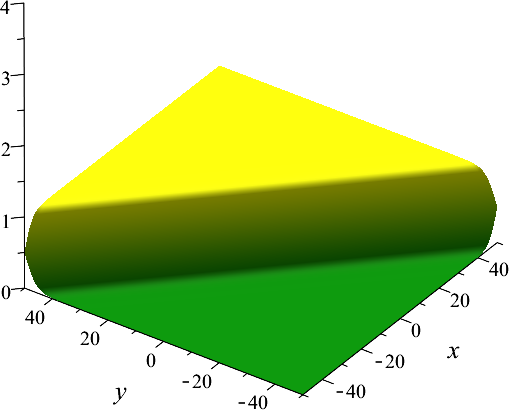
\includegraphics[width=.3\textwidth]{../paper/fig/(3+1)JM-1-soliton.png}    
}
\subfigure[2-孤子解 \label{jm:2-soliton}]{
    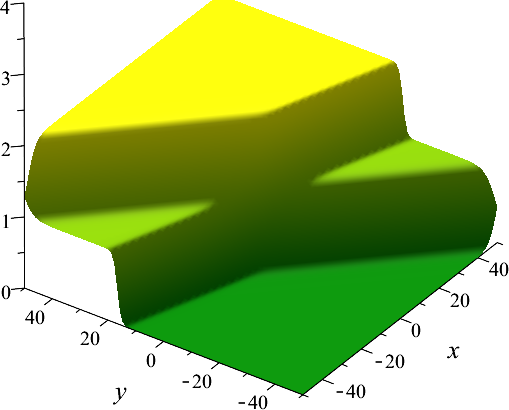
\includegraphics[width=.3\textwidth]{../paper/fig/(3+1)JM-2-soliton.png}
}
\subfigure[3-孤子解 \label{jm:3-soliton}]{
    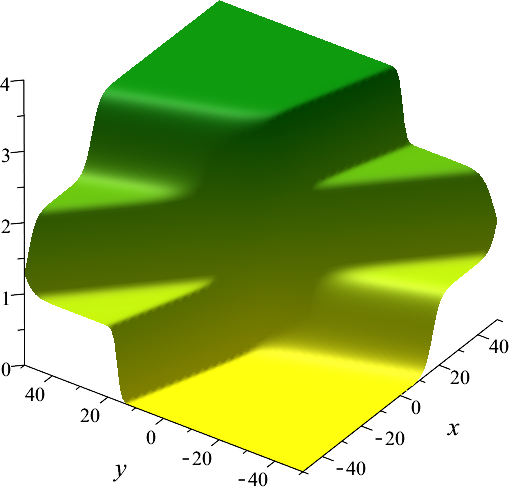
\includegraphics[width=.3\textwidth]{../paper/fig/(3+1)JM-3-soliton.png}
}
\end{figure}
\end{frame}

\subsection{共轭参数法与呼吸子解}
\begin{frame}
\frametitle{共轭参数法与呼吸子解}
\begin{columns}
\begin{column}{0.5\textwidth}
理论:
\[
    f_{m-breather}=\conj{f_{(2m)-soliton}} 
\]
\[
    p_{i,j}=p_{i,j+m}^*,~(j=1,2,\cdots,m)
\]
\[
\begin{split}
    p_{i,j}&=p_{i,j,RE}+I\cdot p_{i,j,IM}, \\ 
    p_{i,j+m}&=p_{i,j,RE}-I\cdot p_{i,j,IM},
\end{split}
\]
\end{column}
\begin{column}{0.5\textwidth}
例子: $m=1,\PS=\bbrace{1,2}$,\\$\xi=k_i(x+p_i y+qz+\omega t)+c$.
\[
\begin{split}
    k_1&=k_{1,RE}+I\cdot k_{1,IM} \\ 
    k_2&=k_{1,RE}-I\cdot k_{1,IM} \\
    p_1&=p_{1,RE}-I\cdot p_{1,IM} \\
    p_2&=p_{1,RE}+I\cdot p_{1,IM} \\ 
\end{split} 
\]
\end{column}
\end{columns}
\end{frame}

\begin{frame}
\begin{figure}
\setcounter{subfigure}{0}
\subfigure[1-呼吸子解 \label{jm:1-breather}]{
    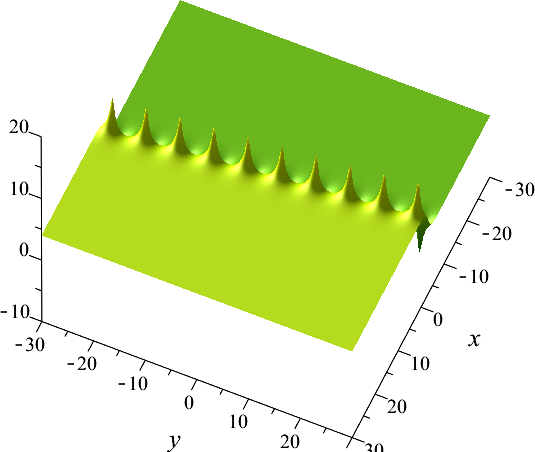
\includegraphics[width=.3\textwidth]{../paper/fig/(3+1)JM-1-breather.png}
}
\subfigure[2-呼吸子解 \label{jm:2-breather}]{
    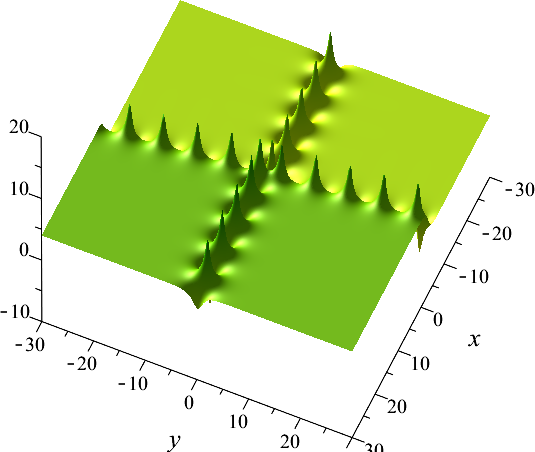
\includegraphics[width=.3\textwidth]{../paper/fig/(3+1)JM-2-breather.png}
}
\subfigure[3-呼吸子解 \label{jm:3-breather}]{
    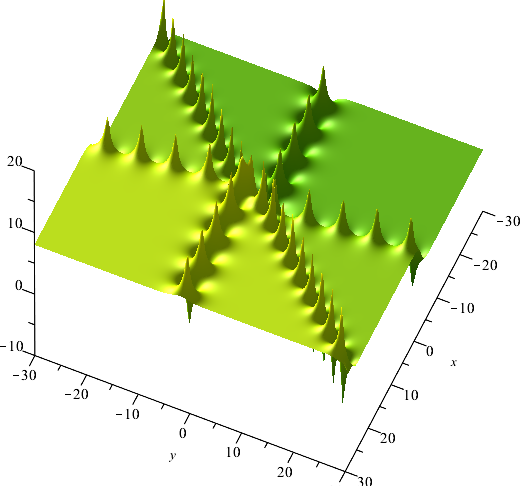
\includegraphics[width=.3\textwidth]{../paper/fig/(3+1)JM-3-breather.png}
}
\subfigure[周期波解 \label{jm:1-periodic}]{
    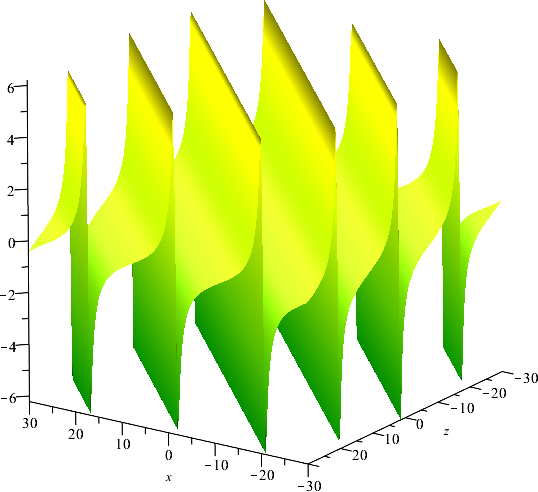
\includegraphics[width=.3\textwidth]{../paper/fig/(3+1)JM-1-periodic.png}
}
\subfigure[孤子-呼吸子相互作用解 \label{jm:soliton-breather}]{
    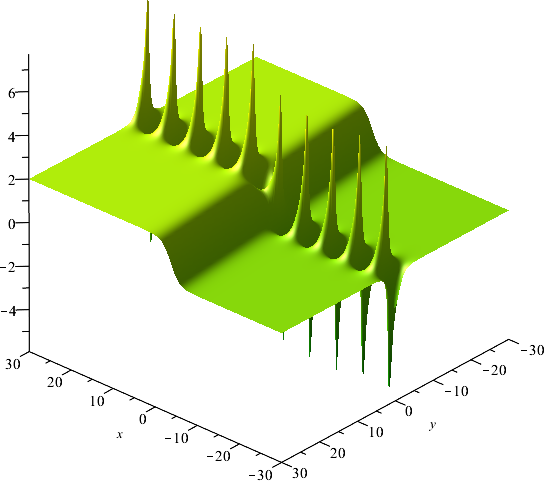
\includegraphics[width=.3\textwidth]{../paper/fig/(3+1)JM-soliton-breather.png}
}
\end{figure}
\end{frame}

\subsection{长极限法与 lump 解}
\begin{frame}{长极限法与 lump 解}
首先, 令
\begin{equation}
\begin{split}
    \xi_i&=k_i\sbrace{x_1+p_ix_2+\cdots+r_ix_n+\omega t}+\xi_i^{(0)},\\
    \eta_i&=\xi_i-\xi_i^{(0)}.
\end{split}
\end{equation}
长极限法的关键在于当$k_i,k_j\rightarrow 0$时, 找到这样两个展开:
\begin{equation}
\begin{split}
    \exp(\eta_i)&=1+k_i \theta_i+o(k_i), \\ 
    h_{i,j}&=1+k_ik_jb_{i,j}+o(k_i^2+k_j^2),
\end{split} \label{lump-expansion}
\end{equation}
其中$o(f)$是Peano余项, 满足$\lim_{f\rightarrow 0}[o(f)/f]=0$.
\end{frame}

\begin{frame}
取$\exp\sbrace{\xi_i^{(0)}}=-1$, 并将上述展开代入到($2m$)-孤子解的生成公式中, 可以得到$m$-lump解. 例如对于一个2-孤子解, 忽略余项后我们有
\begin{equation*}
\begin{split}
\Theta_1&=1+\exp(\xi_1)+\exp(\xi_2)+h_{12}\exp(\xi_1+\xi_2) \\ 
&= 1+\exp(\xi_1)+\exp(\xi_2)+(1+k_1k_2b_{12})\exp(\xi_1+\xi_2) \\ 
&=(1+\exp(\xi_1))(1+\exp(\xi_2))+k_1k_2b_{12}\exp(\eta_1+\eta_2) \\ 
&=(1-(1+k_1\theta_1))(1-(1+k_2\theta_2))+k_1k_2b_{12} \\
&=k_1k_2(\theta_1\theta_2+b_{12}).
\end{split}
\end{equation*}
因为$k_1k_2$是一个能够被TPE消除的常数因子, 所以1-lump解的生成公式为
\begin{equation*}
    \Theta_1=\theta_1\theta_2+b_{12}.
\end{equation*}
\end{frame}
\begin{frame}
推广后可得最终的生成公式为:
\[
    f_{m-lump}=\conj{\Theta_m}
\]
\[
\begin{split}
    \Theta_m&=\prod_{k=1}^{2m}\theta_k+\frac{1}{2}\sum_{i,j}{b_{i,j}}\prod_{J\neq i,j}{\theta_J}+\frac{1}{2! 2^2}\sum_{i,j,k,l}{b_{i,j}b_{k,l}}\prod_{J\neq i,j,k,l}{\theta_{J}}+\cdots \\
    &+\frac{1}{s!2^s}\sum_{i,j,\cdots,u,v}\underbrace{{b_{i,j}b_{k,l}\cdots b_{u,v}}}_{s}\prod_{J\neq i,j,\cdots, u,v}{\theta_J}+\cdots 
\end{split}
\]
例子:
\[
\begin{split}
\Theta_1&=\theta_{1}\theta_{2}+b_{12} \\
\Theta_2&=\theta_{1}\theta_{2}\theta_{3}\theta_{4}+b_{12}\theta_{3}\theta_{4}+b_{13}\theta_{2}\theta_{4}+b_{14}\theta_{2}\theta_{3}+b_{23}\theta_{1}\theta_{4}\\
&+b_{24}\theta_{1}\theta_{3}+b_{34}\theta_{1}\theta_{2}+b_{12}b_{34}+b_{13}b_{34}+b_{14}b_{23}
\end{split}
\]
\end{frame}

\begin{frame}
重写生成公式
\[
    \Theta_m =\sum_{l=0}^m\sum_{s\in L(l)}\sbrace{\prod_{k=1}^l{b_{s_{2k-1},s_{2k}}}\prod_{p\not\in s}{\theta_p}}
\]
\[
    L(l)=\bbrace{\sbrace{s_1, s_2, \cdots ,s_{2l}}\left|s_{2k}>s_{2k-1},s_{2k+1}>s_{2k-1},s_k\in \bbrace{1,\cdots,2l}\right.}
\]
\begin{itemize}
\item $s_{2k}>s_{2k-1}$ 保证了$b_{i,j}=b_{j,i}$的等价情况只出现一次. 
\item $s_{2k+1}>s_{2k-1}$ 保证了$b_{i,j}$的全排列只出现一次.
\end{itemize}
\end{frame}

\begin{frame}
\small
\[
\renewcommand{\arraystretch}{0.8} 
\begin{array}{l}
\Theta_3=\theta_{{1}}\theta_{{2}}\theta_{{3}}\theta_{{4}}\theta_{{5}}\theta_{{6}}
+b_{{12}}\theta_{{3}}\theta_{{4}}\theta_{{5}}\theta_{{6}}
+b_{{13}}\theta_{{2}}\theta_{{4}}\theta_{{5}}\theta_{{6}}
+b_{{14}}\theta_{{2}}\theta_{{3}}\theta_{{5}}\theta_{{6}}\\
+b_{{15}}\theta_{{2}}\theta_{{3}}\theta_{{4}}\theta_{{6}}
+b_{{16}}\theta_{{2}}\theta_{{3}}\theta_{{4}}\theta_{{5}}
+b_{{23}}\theta_{{1}}\theta_{{4}}\theta_{{5}}\theta_{{6}}
+b_{{24}}\theta_{{1}}\theta_{{3}}\theta_{{5}}\theta_{{6}}\\
+b_{{25}}\theta_{{1}}\theta_{{3}}\theta_{{4}}\theta_{{6}}
+b_{{26}}\theta_{{1}}\theta_{{3}}\theta_{{4}}\theta_{{5}}
+b_{{34}}\theta_{{1}}\theta_{{2}}\theta_{{5}}\theta_{{6}}
+b_{{35}}\theta_{{1}}\theta_{{2}}\theta_{{4}}\theta_{{6}}\\
+b_{{36}}\theta_{{1}}\theta_{{2}}\theta_{{4}}\theta_{{5}}
+b_{{45}}\theta_{{1}}\theta_{{2}}\theta_{{3}}\theta_{{6}}
+b_{{46}}\theta_{{1}}\theta_{{2}}\theta_{{3}}\theta_{{5}}
+b_{{56}}\theta_{{1}}\theta_{{2}}\theta_{{3}}\theta_{{4}}\\
+b_{{12}}b_{{34}}\theta_{{5}}\theta_{{6}}
+b_{{12}}b_{{35}}\theta_{{4}}\theta_{{6}}
+b_{{12}}b_{{36}}\theta_{{4}}\theta_{{5}}
+b_{{12}}b_{{45}}\theta_{{3}}\theta_{{6}}
+b_{{12}}b_{{46}}\theta_{{3}}\theta_{{5}}\\
+b_{{12}}b_{{56}}\theta_{{3}}\theta_{{4}}
+b_{{13}}b_{{24}}\theta_{{5}}\theta_{{6}}
+b_{{13}}b_{{25}}\theta_{{4}}\theta_{{6}}
+b_{{13}}b_{{26}}\theta_{{4}}\theta_{{5}}
+b_{{13}}b_{{45}}\theta_{{2}}\theta_{{6}}\\
+b_{{13}}b_{{46}}\theta_{{2}}\theta_{{5}}
+b_{{13}}b_{{56}}\theta_{{2}}\theta_{{4}}
+b_{{14}}b_{{23}}\theta_{{5}}\theta_{{6}}
+b_{{14}}b_{{25}}\theta_{{3}}\theta_{{6}}
+b_{{14}}b_{{26}}\theta_{{3}}\theta_{{5}}\\
+b_{{14}}b_{{35}}\theta_{{2}}\theta_{{6}}
+b_{{14}}b_{{36}}\theta_{{2}}\theta_{{5}}
+b_{{14}}b_{{56}}\theta_{{2}}\theta_{{3}}
+b_{{15}}b_{{23}}\theta_{{4}}\theta_{{6}}
+b_{{15}}b_{{24}}\theta_{{3}}\theta_{{6}}\\
+b_{{15}}b_{{26}}\theta_{{3}}\theta_{{4}}
+b_{{15}}b_{{34}}\theta_{{2}}\theta_{{6}}
+b_{{15}}b_{{36}}\theta_{{2}}\theta_{{4}}
+b_{{15}}b_{{46}}\theta_{{2}}\theta_{{3}}
+b_{{16}}b_{{23}}\theta_{{4}}\theta_{{5}}\\
+b_{{16}}b_{{24}}\theta_{{3}}\theta_{{5}}
+b_{{16}}b_{{25}}\theta_{{3}}\theta_{{4}}
+b_{{16}}b_{{34}}\theta_{{2}}\theta_{{5}}
+b_{{16}}b_{{35}}\theta_{{2}}\theta_{{4}}
+b_{{16}}b_{{45}}\theta_{{2}}\theta_{{3}}\\
+b_{{23}}b_{{45}}\theta_{{1}}\theta_{{6}}
+b_{{23}}b_{{46}}\theta_{{1}}\theta_{{5}}
+b_{{23}}b_{{56}}\theta_{{1}}\theta_{{4}}
+b_{{24}}b_{{35}}\theta_{{1}}\theta_{{6}}
+b_{{24}}b_{{36}}\theta_{{1}}\theta_{{5}}\\
+b_{{24}}b_{{56}}\theta_{{1}}\theta_{{3}}
+b_{{25}}b_{{34}}\theta_{{1}}\theta_{{6}}
+b_{{25}}b_{{36}}\theta_{{1}}\theta_{{4}}
+b_{{25}}b_{{46}}\theta_{{1}}\theta_{{3}}
+b_{{26}}b_{{34}}\theta_{{1}}\theta_{{5}}\\
+b_{{26}}b_{{35}}\theta_{{1}}\theta_{{4}}
+b_{{26}}b_{{45}}\theta_{{1}}\theta_{{3}}
+b_{{34}}b_{{56}}\theta_{{1}}\theta_{{2}}
+b_{{35}}b_{{46}}\theta_{{1}}\theta_{{2}}
+b_{{36}}b_{{45}}\theta_{{1}}\theta_{{2}}\\
+b_{{12}}b_{{34}}b_{{56}}
+b_{{12}}b_{{35}}b_{{46}}
+b_{{12}}b_{{36}}b_{{45}}
+b_{{13}}b_{{24}}b_{{56}}
+b_{{13}}b_{{25}}b_{{46}}
+b_{{13}}b_{{26}}b_{{45}}\\
+b_{{14}}b_{{23}}b_{{56}}
+b_{{14}}b_{{25}}b_{{36}}
+b_{{14}}b_{{26}}b_{{35}}
+b_{{15}}b_{{23}}b_{{46}}
+b_{{15}}b_{{24}}b_{{36}}
+b_{{15}}b_{{26}}b_{{34}}\\
+b_{{16}}b_{{23}}b_{{45}}
+b_{{16}}b_{{24}}b_{{35}}
+b_{{16}}b_{{25}}b_{{34}} .
\end{array}
\]
\end{frame}

\begin{frame}{推导关键参数}
将$\eta$看作是一个关于$k$的函数, 我们有一维泰勒展开  
\begin{equation*}
\begin{split}
\exp(\eta(k))&=\exp(\eta(0))+\eta'(0)\exp(\eta(0))k+o(k)\\ 
&=1+\eta'(0)k+o(k). 
\end{split}
\end{equation*}
从而, 
\begin{equation*}
\theta=\eval{\frac{\partial \eta}{\partial k}}{k=0}=\eval{\frac{\partial \xi}{\partial k}}{k=0}.
\end{equation*}
\end{frame}

\begin{frame}
令$h_{i,j}=h(k_i,k_j)$, 根据对称性我们有$h(x,y)=h(y,x)$. 此外, 取$k_2=0$可以将2-孤子解退化为1-孤子解, 所以$h(k_1,0)=1$. 根据对称性, 我们有$h(0,k_2)=1$. 从而, $h(0,0)=1$, 且
\begin{equation*}
    h_x(0,0)=\eval{\frac{\partial}{\partial x}h(x,0)}{x=0}=0.
\end{equation*}
类似地, 我们有$h_y(0,0)=h_{xx}(0,0)=h_{yy}(0,0)=0$. 因此, $h(x,y)$在$(0,0)$点的二维泰勒展开为 
\begin{equation*}
\begin{split}
h(x,y)&=h(0,0)+h_x(0,0)x+h_y(0,0)y \\ 
&+\frac{1}{2}\mbrace{h_{xx}(0,0)x^2+2h_{xy}(0,0)xy+h_{yy}(0,0)y^2}+o(x^2+y^2) \\ 
&=1+h_{xy}(0,0)xy+o(x^2+y^2).
\end{split}
\end{equation*}
从而, 我们得到
\begin{equation*}
    b_{i,j}=\eval{\frac{\partial^2}{\partial k_i\partial k_j}h_{i,j}}{k_i=0,k_j=0}.
\end{equation*}
\end{frame}

\begin{frame}{关键参数结果}
\begin{columns}
\begin{column}{0.5\textwidth}
关键参数:
\[
\begin{split}
    \theta_i &= \eval{\frac{\partial \xi_i}{\partial p_{1,i}}}{p_{1,i}=0}, \\
    b_{i,j}&= \eval{\frac{\partial^2}{\partial p_{1,i}\partial p_{1,j}}h_{i,j}}{p_{1,i}=0,p_{1,j}=0}.
\end{split}
\]
\end{column}
\begin{column}{0.5\textwidth}
例子: $\PS=\bbrace{1,2}$
\[
\begin{split}
    &\theta_i=\frac{2p_i^2y+(2qz+2x)p_i+3qt}{2p_i}, \\ 
    &b_{i,j}=-\frac{2p_ip_j(p_i+p_j)}{q(p_i-p_j)^2}.
\end{split}
\]
\end{column}
\end{columns}
\end{frame}

\begin{frame}
\begin{figure}
\setcounter{subfigure}{0}
\centering 
\subfigure[1-lump解 \label{jm:1-lump}]{
    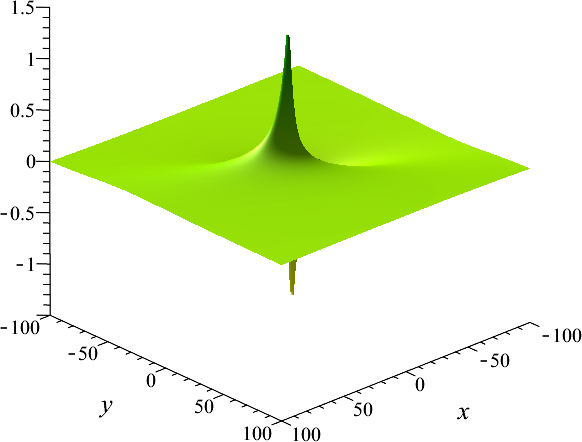
\includegraphics[width=.3\textwidth]{../paper/fig/(3+1)JM-1-lump.png}
}
\subfigure[2-lump解 \label{jm:2-lump}]{
    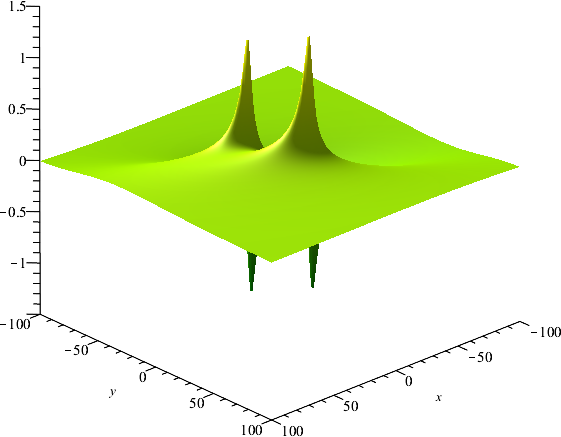
\includegraphics[width=.3\textwidth]{../paper/fig/(3+1)JM-2-lump.png}
}
\subfigure[3-lump解 \label{jm:3-lump}]{
    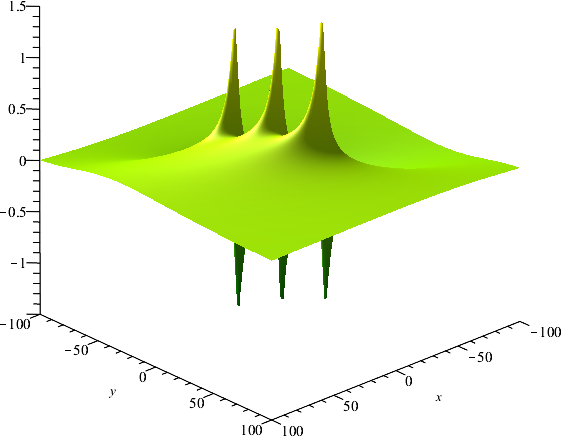
\includegraphics[width=.3\textwidth]{../paper/fig/(3+1)JM-3-lump.png}
}
\subfigure[1-line rogue 解 \label{jm:1-rogue}]{
    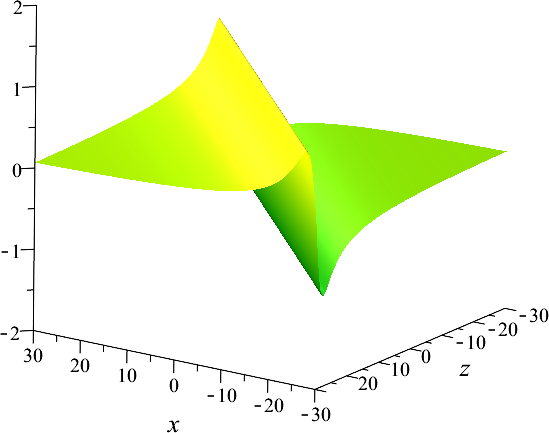
\includegraphics[width=.3\textwidth]{../paper/fig/(3+1)JM-1-rogue.png}
}
\subfigure[2-line rogue 解 \label{jm:2-rogue}]{
    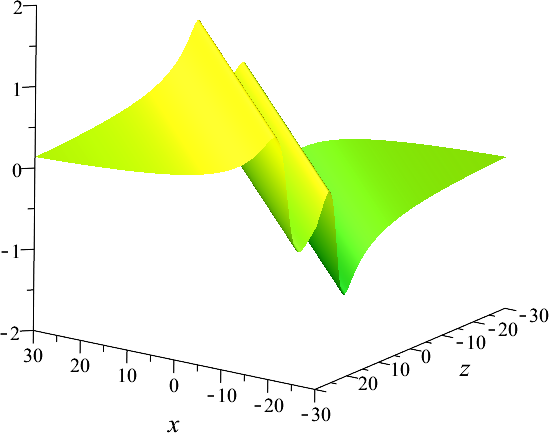
\includegraphics[width=.3\textwidth]{../paper/fig/(3+1)JM-2-rogue.png}
}
\end{figure}
\end{frame}

\subsection{实验与分析}
\begin{frame}
\frametitle{实验与分析}
\begin{columns}
\begin{column}{0.65\textwidth}
\begin{table}
\centering
\small 
\begin{tabular}{lcccc}
\hline
\multicolumn{1}{c}{方程名} & 1 & 12 & 13 & 123 \\ 
\hline
(1+1)KdV & \tpa\tpb & & & \\
(2+1)BKP-T & \tpa\tpb & \tpa\tpa & & \\
(2+1)KP &\tpa\tpb &\tpa\tpa & & \\
(2+1)SK &\tpa\tpb &\tpa\tpa & & \\
(4+1)Fokas-T-2 &\tpa\tpb &\tpa\tpa & & \\
(2+1)CBS & \tpa\tpb & \tpa\tpb & & \\
(2+1)CBS-G & \tpa\tpb & \tpc\tpc & & \\
(3+1)BKP &\tpa\tpb &\tpa\tpa &\tpa\tpa &\tpc\tpc \\
(3+1)KP &\tpa\tpb &\tpa\tpa &\tpa\tpa &\tpc\tpc \\
(3+1)JM &\tpa\tpb &\tpa\tpa &\tpa\tpb &\tpc\tpc \\
(3+1)NEE-T &\tpa\tpb &\tpa\tpa &\tpa\tpb &\tpc\tpc \\
(3+1)YTSF &\tpa\tpb &\tpa\tpa &\tpa\tpb &\tpb\,\tpb \\
(3+1)CBS &\tpa\tpb &\tpa\tpb &\tpa\tpb &\tpa\tpb \\
(4+1)Fokas-T &\tpa\tpb &\tpa\tpb &\tpa\tpb &\tpc\tpc \\
\hline
\end{tabular}
\end{table}
\end{column}
\begin{column}{0.35\textwidth}
\begin{itemize}
\item `\tpa{}' 表示能够满足原方程.
\item `\tpb{}' 表示不能得到解.
\item `\tpc{}' 表示有解但不满足原方程.
\item 第一个对应3孤子解, 第二个对应2 lump解.
\end{itemize}
\end{column}
\end{columns}
\end{frame}

\begin{frame}
实验结果:
\begin{itemize}
\item $\PS=\bbrace{1}$, 所有方程都有3-孤子解. 
\item $\PS=\ALLP$, 除了两个CBS方程, 所有(2+1)维的方程都有lump解. 
\item $\PS=\ALLP$, (3+1)YTSF方程没有孤子解, 所以不能先取$\PS=\ALLP$, 再取特殊值使得$\PS\subsetneq \ALLP$. 
\item 大部分(3+1)维方程在$\PS=\bbrace{1,2}$或$\PS=\bbrace{1,3}$是才有孤子解和lump解.
\item 孤子解成立是lump解成立的必要条件. 
\end{itemize}
\end{frame}

\subsection{软件展示}
\begin{frame}{软件展示}
\href{run:../LypReportProgram/TwSolver.mw}{TwSolver.mw}
\begin{itemize}
\item (3+1)JM 方程, 整体流程和绘图结果展示.
\item (2+1)BKP 方程, 积分预处理和\Painleve{}展开结果的选择, 以及不同的绘图方式展示.
\item (4+1)Fokas 方程, 高维方程降维求解的例子.
\end{itemize}
\end{frame}

\begin{frame}{$n$阶展开方法}
齐次平衡原则是很多算法的基础, 如双曲正切方法、Painlev\'e 截断展开法、 Jacobi椭圆函数方法等. 我们以双曲正切方法为例来展示$n$解展开方法对齐次平衡原则的进一步完善. 
\end{frame}



% \begin{frame}{$n$阶展开方法构造新的双曲正切函数解}
% \begin{enumerate}
% \item 双曲正切方法
% \item 三类平衡点
% \item $n$阶展开多项式的性质
% \item 例1: (4+1)Fokas 方程三类平衡点都有
% \item 例2: (1+1)EMM 方程第三类平衡点的决定性作用 
% \item 例3: 上界的作用
% \end{enumerate}
% \end{frame}

\begin{frame}{双曲正切方法}
考虑非线性演化方程 
\[
    U\sbrace{u,u\up{1},u\up{2},\cdots}=0, 
\]
其中$u=u(x_1,\cdots,x_d)$, 而$u\up{k}$表示$u$的所有$k$阶导数的集合, 例如$u\up{1}=\bbrace{u_{x_1},\cdots,u_{x_d}}$. 
将
\[
    u=\sum_{k=0}^{m}{a_k\tanh^k(\xi)}
\]
代入原方程后, 方程中各个加法项都是关于$\tanh(\xi)$的多项式, 设各项的次数分别为 
\[
    s_1 m+d_1,\cdots,s_l m + d_l . 
\]
\end{frame}

\begin{frame}{三类平衡点}
在齐次平衡原则中, 以往通过
\[
    s_i m+d_i=s_j m+d_j, s_i\neq s_j , m\in \mathbb Z_+. 
\]
来确定$m$的值, 没有考虑$s_i=s_j$的情况. 但是我们不能否定该情况下平衡的可能性, 所以我们重新定义平衡的条件如下:
\begin{itemize}
    \item 整数性: $ m\in \mathbb Z_+$ 
    \item 平衡性: $\exists i\neq j, s_i m+d_i=s_j m+d_j $
    \item 最大性: $\forall k \not\in \bbrace{i,j}, s_i m+d_i\ge s_k m+d_k $
\end{itemize}
\end{frame}

\begin{frame}
\begin{columns}
\begin{column}{.5\textwidth}
\begin{figure}
\centering
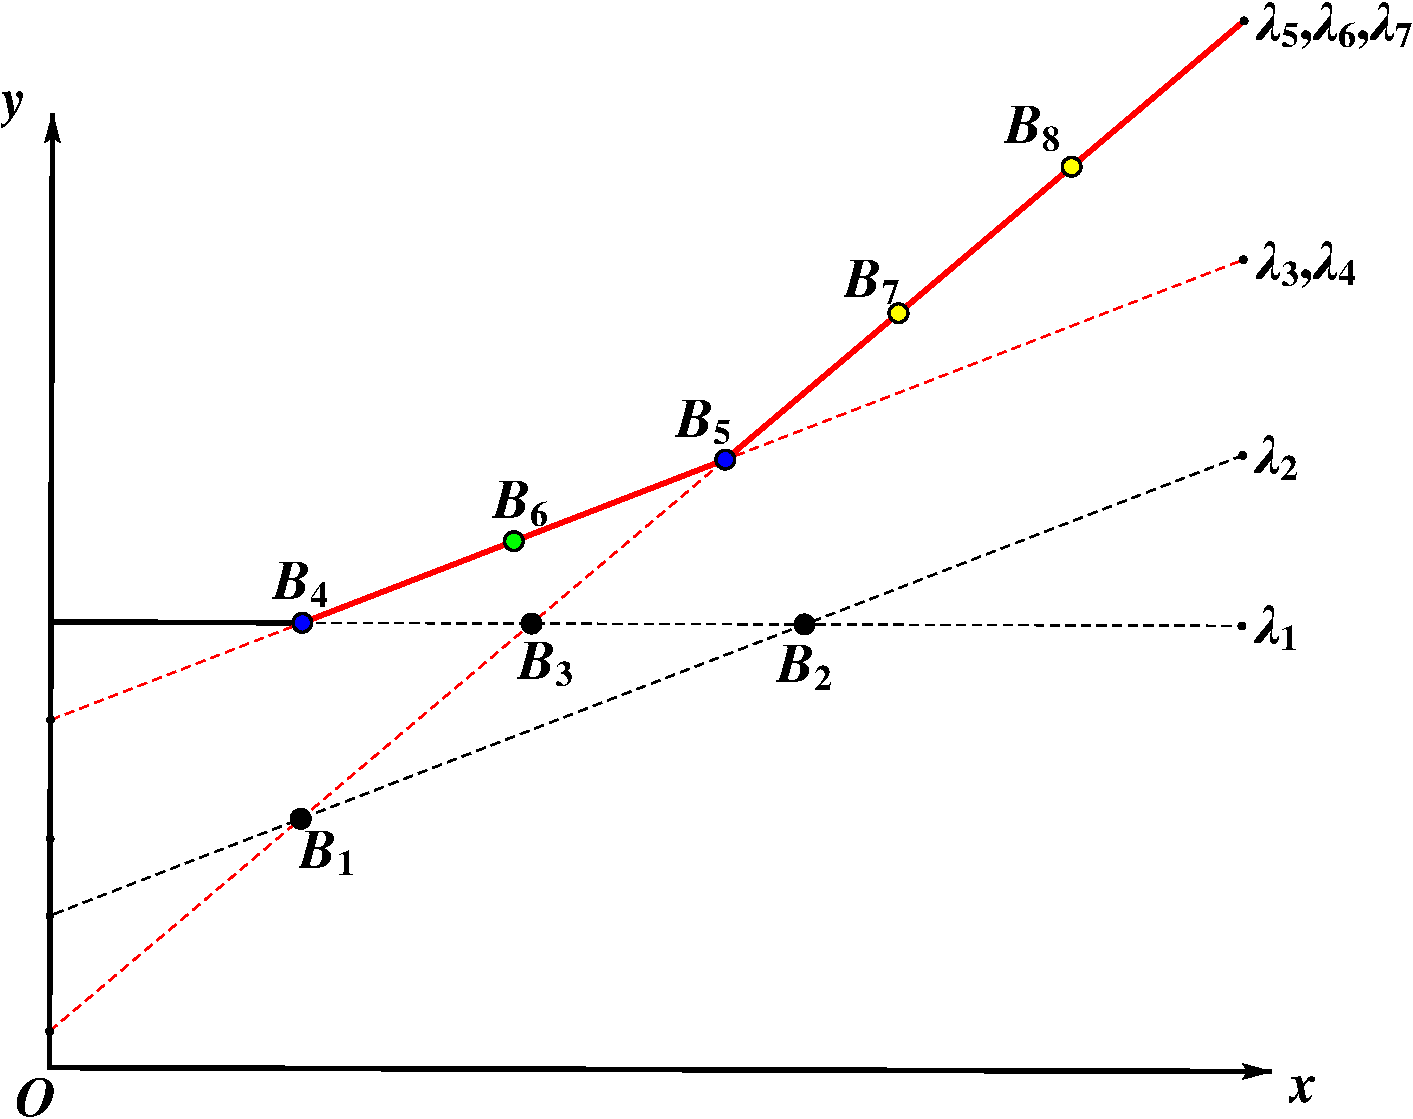
\includegraphics[width=\textwidth]{../paper/fig/ps.pdf}
\caption{平衡点分类示意图}
\end{figure}
\end{column}
\begin{column}{.5\textwidth}
\[
    \lambda_k = s_k m + d_k 
\]
\begin{itemize}
\item $B_1,B_2,B_3$不满足最大性条件, 不是平衡点. 
\item $B_4,B_5$可以由平衡性条件唯一确定, 是\textbf{第一类平衡点}. 
\item $B_6$不能由平衡性条件唯一确定, 但是可以由最大性条件确定, 是\textbf{第二类平衡点}.
\item $B_7,B_8$以及右侧的一系列整点, 满足三种平衡条件, 但无法确定其上界, 是\textbf{第三类平衡点}. 所以我们提出了$n$阶展开方法来确定此类平衡点的上界. 
\end{itemize}
\end{column}
\end{columns}
\end{frame}

\begin{frame}{$n$阶展开方法}
\small
因为求导会使得$m$出现在系数中, 所以我们可以通过方程最高$n$项的系数来分析$m$的上界, 所以我们提出了$n$阶展开方法. 

考虑一个关于$x$的$m$次多项式, 其$n$阶展开形式为
\[
    F\sbrace{x,m,u\up n}=\sum_{k=0}^{n-1}{u_k x^{m-k}}+\OO\sbrace{x^{m-n}},
\]
其中 
\[
\OO\sbrace{x^n}=\left\{
\begin{array}{cl}
\text{次数不超过}\,n\,\text{的多项式} & n\ge 0, \\
0                                    & n<0 .
\end{array}
\right.
\]
在双曲正切方法中, 取
\[
    u=F\sbrace{\tanh(\xi),m,a\up{n}}=\sum_{k=0}^{n-1}{a_k \tanh^{m-k}(\xi)}+\OO(\tanh^{m-n}(\xi))
\]
代入原方程, 将方程转化为关于$\tanh(\xi)$的$n$阶展开多项式, 所以我们要考虑$n$阶展开多项式的乘法, 求导和加法的规则. 
\end{frame}

% \begin{frame}{$n$阶展开多项式的性质}
% \begin{itemize}
% \item $n$阶展开多项式的相乘还是$n$阶展开多项式.
% \item $n$阶展开多项式求导后, 其系数中将会包含$m$.
% \item $n$阶展开多项式加法的约束条件.
% \end{itemize}
% \end{frame}

\begin{frame}{$n$阶展开多项式的乘法}
\[
\begin{aligned}
& F\sbrace{x,m,u \up n}\cdot F\sbrace{x,l,v\up n} \\
=& \mbrace{\sum_{k=0}^{n-1}{u_k x^{m-k}}+\OO\sbrace{x^{m-n}}}\mbrace{\sum_{k=0}^{n-1}{v_k x^{l-k}}+\OO\sbrace{x^{l-n}}} \\
=& \mbrace{\sum_{k=0}^{n-1}{u_k x^{m-k}}}\mbrace{\sum_{k=0}^{n-1}{v_k x^{l-k}}}+\OO\sbrace{x^{m+l-n}} \\
=& \sum_{p=0}^{n-1}{x^{m+l-p}\mbrace{\sum_{k=0}^p{u_k v_{p-k}}}}+\OO\sbrace{x^{m+l-n}} \\
=& F\sbrace{x,m+l,w\up n} 
\end{aligned} 
\]
\end{frame}

\begin{frame}{$n$阶展开多项式的求导}
\[
\begin{aligned}
& \DIF{t}F\sbrace{x,m,u\up{n}}  \\
=& \DIF{t}\sbrace{\sum_{k=0}^{n-1}{u_k x^{m-k}}+\OO(x^{m-n})} \\
=& \sum_{k=0}^{n-1}{\DIFF{u_k}{t}x^{m-k}}+\DIFF{x}{t}\cdot\sum_{k=0}^{n-1}{u_k (m-k) x^{m-k-1}}+\DIFF{x}{t}\cdot\OO(x^{m-n-1}) \\
=& \sum_{k=0}^{n-1}{\DIFF{u_k}{t}x^{m-k}}+\DIFF{x}{t}\cdot\sbrace{\sum_{k=0}^{n-1}{u_k (m-k) x^{(m-1)-k}}+\OO\sbrace{x^{(m-1)-n)}}} \\ 
=& F\sbrace{x,m,v\up{n}}+\DIFF{x}{t}\cdot F\sbrace{x,m-1,w\up{n}} 
\end{aligned}
\]
\end{frame}


\begin{frame}{$n$阶展开多项式的加法}
考虑加法 
\[
    F\sbrace{x,s_i m+d_i,u\up n}+F\sbrace{x,s_j m+d_j,v\up n}
\]  
因为我们无法比较$s_i m + d_i$ 和 $s_j m + d_j$ 大小, 所以无法直接求和. 

假设$F\sbrace{x,s_j m+d_j,v\up n}$在求和时不会影响$F\sbrace{x,s_i m+d_i,u\up n}$的前$n$项, 则需 
\[
    s_i m+d_i - n > s_j m+d_j 
\]
从而 
\[
\begin{aligned}
&F\sbrace{x,s_i m+d_i,u\up n}+F\sbrace{x,s_j m+d_j,v\up n} \\
=&\left\{
\begin{array}{cl}
    F\sbrace{x,s_i m+d_i,u\up n} & s_i>s_j,            \\
    F\sbrace{x,s_i m+d_i,w\up n} & s_i=s_j.
\end{array}
\right.
\end{aligned}
\]
\end{frame}

\begin{frame}{确定第三类平衡点的上界}    
\small 
将$F\sbrace{\tanh(\xi),m,a\up{n}}$代入原方程, 则原方程的$n$阶展开形式为
\[
    F\sbrace{\tanh(\xi),\sigma m+\delta,\Omega\up{n}}=0 .
\]
设$\Omega_{k}$是第一个非零项的系数, 则: 

(一) $\Omega_{k}=0$关于$m$有正整数解, 此时$m$的上界为
\[
    m_{31}=\max\bbrace{m\in \mathbb Z_+|\Omega_{k}=0}.
\]

(二) $\Omega_{k}=0$关于$m$没有正整数解, 这说明若加法的假设条件成立, 则原方程无解. 所以需要加法的假设条件不成立才可能有解, 此时需要满足 
\[
    \forall s_j<\sigma, \sigma m + \delta - k \le s_j m + d_j
\]
则有
\[
    m\le m_{32} = \underset{s_j<\sigma}{\max}{\frac{d_j-\delta+k}{\sigma-s_j}}
\]
最终, 第三类平衡点的上界为 
\[
    m_3 = \max\bbrace{m_{31},m_{32}}. 
\]
\end{frame}

\begin{frame}{示例}
下面我们通过三个实例来说明$n$阶展开方法的思路和步骤. 

\end{frame}

\begin{frame}{例1: (4+1)Fokas方程(含全部三类平衡点)}
% \small 
\begin{equation*}
    u_{tx}-\frac{1}{4}u_{xxxy}+\frac{1}{4}u_{xyyy}+3u_xu_y+3uu_{xy}-\frac{3}{2}u_{wz}=0 ,
\end{equation*}
其阶数列表为$\mbrace{m+2,m+4,m+4,2m+2,2m+2,m+2}$. 
\begin{itemize}
\item 首先由最大性原则, 上述列表可以简化为\[\mbrace{m+4,m+4,2m+2,2m+2}\]
\item 然后考虑第一类平衡点, 根据$2m+2=m+4$可以得到$m=2$.
\item 然后考虑第二类平衡点, 考虑$m+4=m+4$, 根据最大性约束有$m+4>2m+2$, 可得$m<2$, 所以有第二类平衡点$m=1$.
\end{itemize}
\end{frame}

\begin{frame}
因为有两个$2m+2$, 所以接下来考虑第三类平衡点. 首先作行波变换$\xi=kx+py+qz+rw+ct+\eta$, 然后将 $F\sbrace{\tanh(\xi),m,a\up{n}}$ 代入原方程可以得到 
\begin{equation*}
\begin{aligned}
0&=24kpa_0^2m\sbrace{m+\frac{1}{2}}\tanh^{2m+2}(\xi)\\ 
&+24\,k\,m\,p\,{{a}_{0}}\,{{a}_{1}}\,\left( 2\,m-1\right)\tanh^{2m+1}(\xi)+\OO\sbrace{\tanh^{2m}(\xi)} . 
\end{aligned}
\end{equation*}
因为$\Omega_0=24kpa_0^2m\sbrace{m+\frac{1}{2}}=0$关于$m$没有正整数解, 所以需要
\[2m+2-0\le m+4,\]
从而得到第三类平衡点的上界为$m=2$.

\end{frame}

\begin{frame}
综合以上三类平衡点, 我们得到$m$的上界为2, 将
\[
    u=\sum_{k=0}^2{a_k\tanh^k(\xi)}
\]
代入原方程, 令$\tanh$的不同次幂项的系数为零, 可以得到一个非线性代数方程组, 求解该方程组并返回原来的变量, 可以得到原方程的一个解
\begin{equation*}
\begin{aligned}
    u&=\frac{\left( -4\,{k}^{3}\,p+4\,k\,{p}^{3}-2\,c\,k+3\,q\,r\right) }{6\,p\,k} \\ 
    &+\left( {k}^{2}-{p}^{2}\right) \,\left( \tanh\left( c\,t+k\,x+p\,y+q\,z+r\,w+\eta\right) \right) ^{2}
\end{aligned}
\end{equation*}
\end{frame}

\begin{frame}{例2: (1+1)维方程(无第一,二类平衡点)}
\begin{equation*}
    {{u}_{t}}+{{u}_{x}}+\alpha\,{{u}_{xxx}}+\beta\,u\,{{u}_{x}}+\gamma\,u\,{{u}_{xxx}}+\delta\,{{u}_{x}}\,{{u}_{xx}}=0,
\end{equation*}
该方程是从弹性介质的微观结构中导出的, 其阶数列表为
\[
    [m+1,m+1,m+3,2m+1,2m+3,2m+3],
\]
由最大性条件, 上述列表可简化为 
\[
    [m+3,2m+3,2m+3], 
\]
所以该方程不存在第一,二类平衡点, 只可能存在第三类平衡点.  作行波变换$\xi=kx+ct+\eta$, 然后将 $F\sbrace{\tanh(\xi),m,a\up{n}}$ 代入原方程可以得到 
\begin{equation*}
    \Omega_0=-{{{a}_{0}}}^{2}\,{k}^{3}\,m\,\left( m+1\right) \,\left( m\,\delta+\gamma\,m+2\,\gamma\right)
\end{equation*}
可得 $m=0$, 原方程没有非平凡的解. 当$m=\frac{-2 \gamma}{\gamma+\delta}$为正整数时, 就存在其它可能的平衡点.
\end{frame}

\begin{frame}
当$\gamma=-1,\delta=3$时, $m=1$, 可获得原方程的两个解 
\[
    u=\alpha+a_1\tanh\sbrace{\pm\sbrace{\frac{\sqrt{\beta}}{2}x-\frac{\sqrt{\beta}(\alpha \beta+1)}{2}t}+\eta}. 
\]

此外, 我们总结出: 当$n\ge 1$时, 若$\gamma=-n,\delta=n+1$, 则$m=2n$, 原方程有解 
\begin{equation*}
u=(-1)^n a_{2n} \sbrace{\tanh^2\sbrace{\pm\sbrace{\frac{\sqrt{-\beta}}{2n}x-\frac{\sqrt{-\beta}(\alpha\beta+n)}{2n^2}t}+\eta}-1}^n+\frac{\alpha}{n} .
\end{equation*}
\end{frame}

\begin{frame}{例3: 一般五阶模型}
\[
    u_t+\sbrace{\alpha\,{{{u}_{x}}}^{2}+\beta\,u\,{{u}_{xx}}+\mu\,{{u}_{xx}}+{{u}_{xxxx}}+p\,u+q\,{u}^{2} }_x = 0
\]
取$\alpha=5,\beta=-4$, 则其阶数列表为 
\[
    \mbrace{m+1,2m+3,2m+3,m+3,m+5,m+1,2m+1} .
\]
由最大性条件, 上述列表可简化为 
\[
    \mbrace{2m+3,2m+3,m+5}
\]
首先考虑第一类平衡点, 由$2m+3=m+5$可得$m=2$.
然后考虑第三类平衡点, 做行波变换$\xi=kx+ct+\eta$, 我们有 
\[
    \Omega_0 = -2k^3a_0^2m(m+1)(m-4) 
\]
$\Omega_0=0$有正整数解$m=4$
\end{frame}

\begin{frame}
此时, 原方程有两个解:
\[
\begin{aligned}
u&=30\,{k}^{2}\,{T}^{2}-20\,{k}^{2}+\frac{\mu}{4}+\frac{5\,q}{4} \\
T&=\tanh\left( \frac{k\,\left( 288\,{k}^{4}-\mu\,q-5\,{q}^{2}-2\,p\right) \,t}{2}+k\,x+\eta\right)
\end{aligned}
\]
和
\[
\begin{aligned}
u&=\frac{{-3360\,{k}^{4}\,{T}^{4}+6720\,{k}^{4}\,{T}^{2}-2528\,{k}^{4}+16\,{k}^{2}\,\mu+52\,{k}^{2}\,q+\mu\,q}}{64\,{k}^{2}+4\,q}\\ 
T&=\tanh\left( \frac{k\,\left( 1152\,{k}^{4}-52\,{k}^{2}\,q-\mu\,q-2\,p\right) \,t}{2}+k\,x+\eta\right) 
\end{aligned}
\]
\end{frame}

% \begin{frame}
% \frametitle{直接代数方法求$n$-孤子与1-lump的相互作用解}
% \begin{enumerate}
% \item NS1L: 求$n$-孤子-1 lump相互作用解的软件包
% \item PGSolve: 分组并行算法
% \item 应用实例: (3+1)YTSF 方程
% \item 求解效率对比
% \item 软件展示 
% \end{enumerate}
% \end{frame}

\begin{frame}{直接代数方法求相互作用解}
考虑非线性演化方程
\[
    U(u,u\up{1},u\up{2},\cdots)=0 
\]
其中 $u=u(x_1,\cdots,x_m)$. 假设原方程存在 Painleve 截断展开  
\[
    u=\sum_{k=1}^m{\frac{u_k}{f^{m-k+1}}}
\]
基于$n$阶展开方法, 我们可以确定$m$的上界, 从而确定这个变换的具体表达式. 将上述变换代入原方程, 可以得到关于$f$及其导数的方程
\[
    F(f,f\up{1},f\up{2},f\up{3}\cdots)=0
\]
直接代数方法的思路: 给定$f$的假设形式之后, 代入上述方程后, 合并同类项, 并令不同次幂项的系数为零, 得到一个非线性代数方程组. 
\end{frame}

\begin{frame}{求解非线性代数方程组的新算法}
对于高维方程, 相互作用解的假设形式越复杂, 得到的非线性代数方程组的规模越大. 且随解的阶数增长, 其规模急速增长 . Csolve 的特点是不增解不漏解,这样,一旦一个分支方程组求不出来,则我们得不到任何解.故对大规模非线性代数方程组(几百个方程), 我们采用以下两种策略: 

\begin{itemize}
\item 分组并行求解算法: 当遇到长时间算不动的分支时, 我们可以舍弃它. 同时, 我们还能通过指定条件, 来舍去平凡解的分支.  
\item 继承求解算法: 将低阶解作为高阶解的初始解, 能迅速降低高阶解对应的非线性代数方程组的规模. 
\end{itemize}


\end{frame}

\begin{frame}
我们以计算$n$-孤子和1-lump的相互作用解为例.

在上述简单 Hirota 方法中, $n$-孤子解的形式为
\[
    f_{n-soliton}=\sum_{R\subseteq \bbrace{1,\cdots,n}}\mbrace{\sbrace{\prod_{\bbrace{i,j}\subseteq R}{h_{i,j}}}\exp\sbrace{\sum_{k\in R}{\xi_k}}} . 
\]
1-lump解的形式为 
\[
    f_{1-lump}=\theta_1\theta_2+b_{12}, 
\]
其中$\theta_1,\theta_2$互为共轭, 所以它能写成
\[
    f_{1-lump}=\xi_1^2+\xi_2^2+b_{12} . 
\]
\end{frame}

\begin{frame}
\small 
从而我们假设$n$-孤子和1-lump 相互作用解的$f$具有如下形式 
\[
    f_n=\sbrace{\xi_1+\eta_1}^2+\sbrace{\xi_2+\eta_2}^2+\sum_{i=1}^{2^n}\sbrace {q_i\prod_{k \in T_i}{\exp(\xi_{k+2})}}
\]
\[
    \xi_k=\sum_{j=1}^m{p_{j,k}x_j}=p_{1,k}x_1+\cdots+p_{m,k}x_m
\]
其中$\eta_1,\eta_2$是常量, $T_i$是$\bbrace{1,2,\cdots,n}$的第$i$个子集. 子集顺序为
\[
    \emptyset,\bbrace{1},\bbrace{2},\bbrace{1,2},\bbrace{3},\bbrace{1,3},\bbrace{2,3},\bbrace{1,2,3},\cdots 
\]
从而, 高阶解能够退化为相同形式的低阶解, 这是能够继承求解的前提条件. 例如, 
\[
\begin{aligned}
    f_0 &= \sbrace{\xi_1+\eta_1}^2+\sbrace{\xi_2+\eta_2}^2+q_1\\ 
    f_1 &= \sbrace{\xi_1+\eta_1}^2+\sbrace{\xi_2+\eta_2}^2+q_1+q_2 \exp(\xi_3) \\ 
    f_2 &= \sbrace{\xi_1+\eta_1}^2+\sbrace{\xi_2+\eta_2}^2+q_1+q_2 \exp(\xi_3) \\
        & +q_3 \exp(\xi_4) + q_4 \exp(\xi_3+\xi_4)
\end{aligned}
\]
继承求解的思路: 将$f_0$的解作为$f_1$的初始解继续求解, 以此类推.
\end{frame}

\begin{frame}
约束条件:
\begin{itemize}
\item 孤子解的各个相互作用系数非零.
\item 行波中各个变量的系数不能全为零. 
\item lump 解部分不退化.
\item 孤子解部分不退化. 
\end{itemize}
相应的避免取值集合为: 
\[
\begin{aligned}
    S&=\bbrace{\bbrace{q_i=0}|2\le i \le 2^n} \\ 
        &\cup \bbrace{\bbrace{p_{1,k}=0,\cdots,p_{m,k}=0}|1\le k \le n+2}  \\
        &\cup \bbrace{\bbrace{p_{j,1}=0,p_{j,2}=0}|1\le j \le m} \\ 
        &\cup \bbrace{\bbrace{p_{j,3}=0,\cdots,p_{j,n+2}=0}|1\le j \le m} .  
\end{aligned}
\]
对于一个解$sol$ (是一个集合), 若存在$s\in S$, 满足$s\subseteq sol$, 则$sol$就不是我们想要的解.
\end{frame}



\begin{frame}
\frametitle{分组并行求解算法}
\begin{figure}
\centering
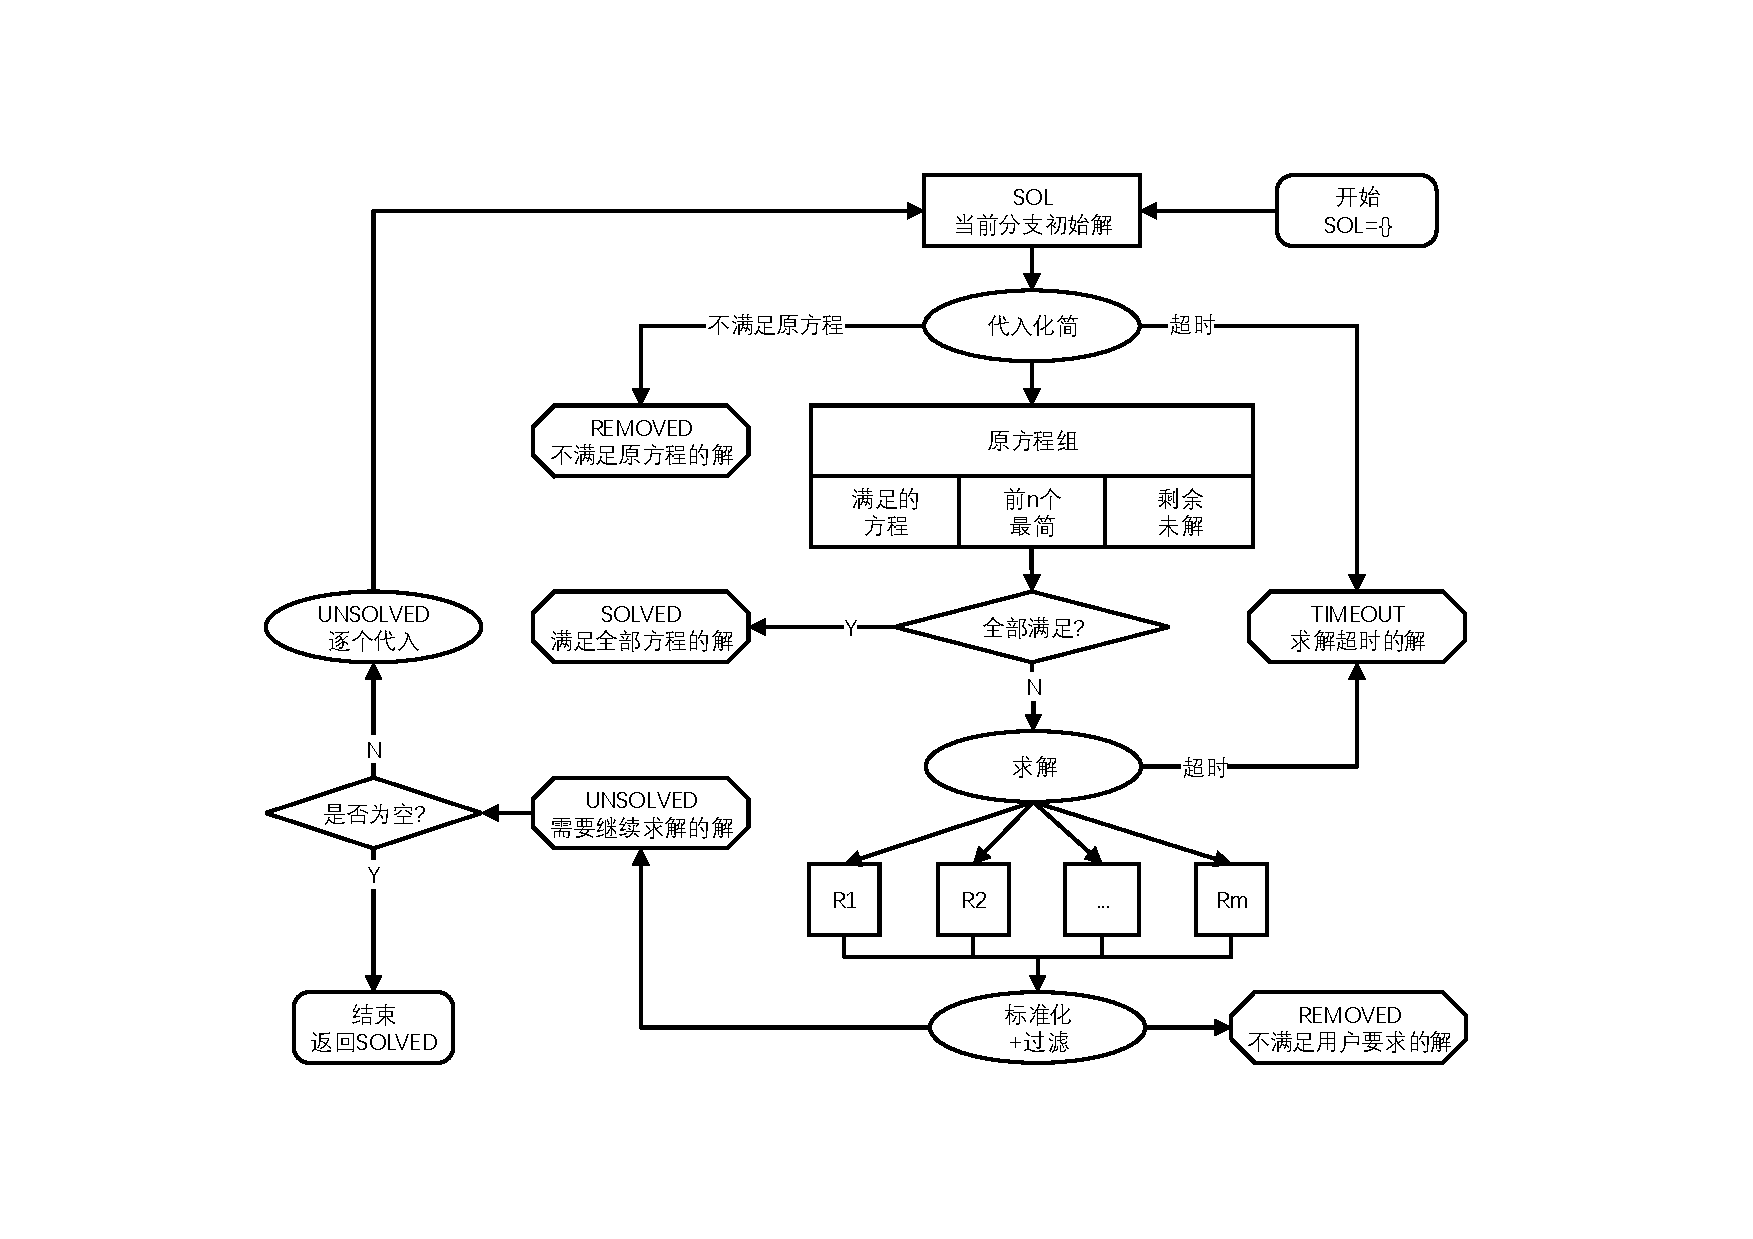
\includegraphics[height=0.8\textheight]{../paper/fig/pgsolve.pdf}
\end{figure}
\end{frame}

\begin{frame}
代入化简所有方程的优势:
\begin{enumerate}
\item 对尚未求解的方程进行代入化简, 能够对新的方程组按照复杂度重新排序, 从而获得更简单的方程.
\item 对已经求解过的方程进行代入化简, 能够验证当前分支的解是否满足这部分方程. 
\item 虽然单个分组只求解了$n$个方程, 但是获得的解可能满足更多的方程, 代入后可以及时地减少待求解方程的数量. 
\end{enumerate}
\end{frame}

\begin{frame}{应用实例: (3+1)YTSF 方程}
\[
    3\,\alpha\,u_{{{\it yy}}}+4\,u_{{x}}u_{{{\it xz}}}+2\,u_{{{\it xx}}}u_{{z}}-4\,u_{{{\it tx}}}+u_{{{\it xxxz}}}=0. 
\]
在接下来的例子中, 分组大小 $n=5$. 

% \[
% \begin{aligned}
%     f_0 &=\sbrace{\xi_1+\eta_1}^2+\sbrace{\xi_2+\eta_2}^2 \\ 
%     f_1 &= \sbrace{\xi_1+\eta_1}^2+\sbrace{\xi_2+\eta_2}^2+q_1+q_2 \exp(\xi_3) \\ 
%     f_2 &= \sbrace{\xi_1+\eta_1}^2+\sbrace{\xi_2+\eta_2}^2+q_1+q_2 \exp(\xi_3) \\
%         & +q_3 \exp(\xi_4) + q_4 \exp(\xi_3+\xi_4)
% \end{aligned}
% \]
\end{frame}
\begin{frame}
\begin{figure}
\centering
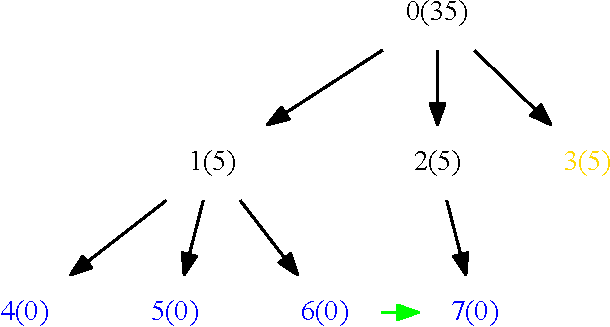
\includegraphics[width=.5\textwidth]{../paper/fig/0S1L.pdf}
\caption{0S-1L 求解分支图 (1秒)}
\end{figure}
\end{frame}

\begin{frame}
因为lump解中$\xi_1+\eta_1$和$\xi_2+\eta_2$是对称的, 所以我们消去了一个等价的解, 得到两组解:
\small 
\[
\begin{aligned}
\dbrace{
& p_{{31}}={\frac {p_{{11}}p_{{32}}}{p_{{12}}}}, 
p_{{41}}={\frac {3\alpha \left(  \left( {p_{{21}}}^{2}-{p_{{22}}}^{2} \right) p_{{11}}+2p_{{12}}p_{{21}}p_{{22}} \right) }{4{p_{{11}}}^{2}+4{p_{{12}}}^{2}}}, \\
& p_{{42}}={\frac {3\alpha \left( 2p_{{11}}p_{{21}}p_{{22}}-p_{{12}}{p_{{21}}}^{2}+p_{{12}}{p_{{22}}}^{2}\right) }{4{p_{{11}}}^{2}+4{p_{{12}}}^{2}}}, 
q_{{1}}=-{\frac {p_{{32}} \left( {p_{{11}}}^{2}+{p_{{12}}}^{2} \right) ^{3}}{\alpha p_{{12}} \left( p_{{11}}p_{{22}}-p_{{12}}p_{{21}} \right) ^{2}}} 
} 
\end{aligned}
\]
\[
 \left\{ p_{{12}}=0,p_{{31}}=-{\frac {\alpha q_{{1}}{p_{{22}}}^{2}
}{{p_{{11}}}^{3}}},p_{{32}}=0,p_{{41}}={\frac {3\alpha
 \left( {p_{{21}}}^{2}-{p_{{22}}}^{2} \right) }{4p_{{11}}}},p_{{42}
}={\frac {3\alpha p_{{21}}p_{{22}}}{2p_{{11}}}} \right\}
\]
    
\end{frame}


\begin{frame}
\begin{figure}
\centering
\setcounter{subfigure}{0}
\subfigure[]{
    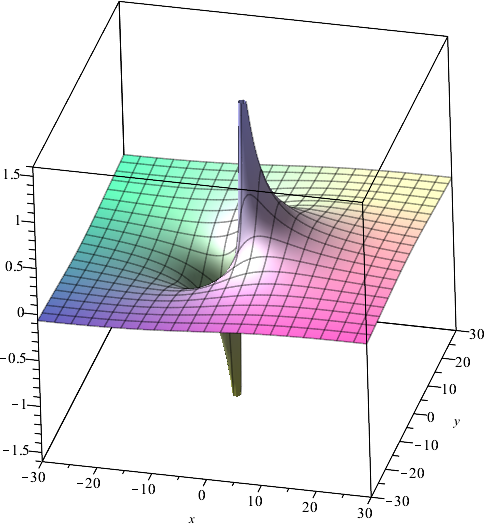
\includegraphics[width=.3\textwidth]{../paper/fig/0S1L-1.png}
}
\subfigure[]{
    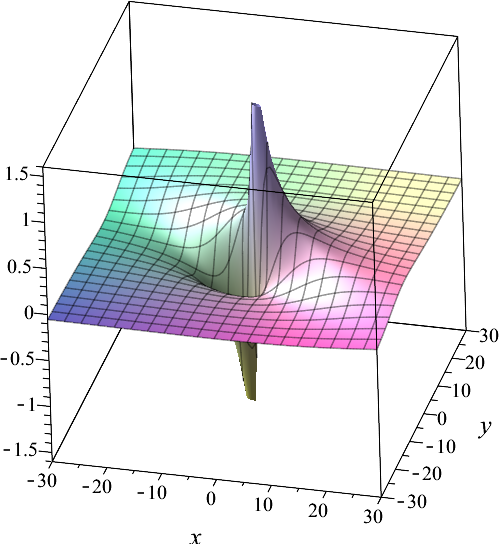
\includegraphics[width=.3\textwidth]{../paper/fig/0S1L-2.png}
}
\caption{(3+1)维 YTSF 方程的 0S-1L 解}
\end{figure}
\end{frame}

\begin{frame}
接下来继续求 1S-1L 解, 下面通过图示比较直接求解与继承求解的效率差异. 

\[
\begin{aligned}
    f_0 &= \sbrace{\xi_1+\eta_1}^2+\sbrace{\xi_2+\eta_2}^2+q_1\\ 
    f_1 &= \sbrace{\xi_1+\eta_1}^2+\sbrace{\xi_2+\eta_2}^2+q_1+q_2 \exp(\xi_3) 
\end{aligned}
\]
\end{frame}

\begin{frame}
\begin{figure}
\centering
\setcounter{subfigure}{0}
\subfigure[1S-1L直接求解(8秒)]{
    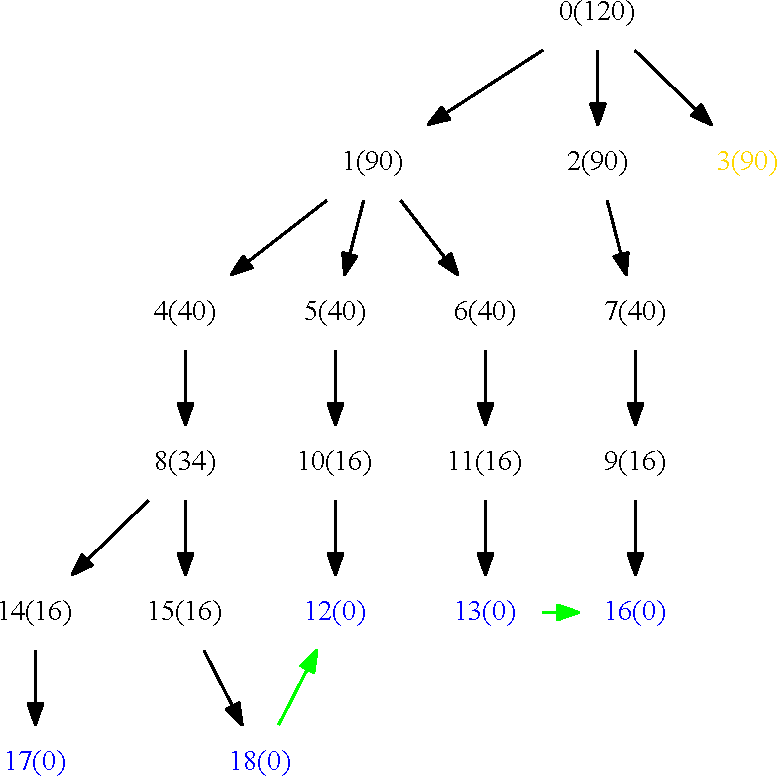
\includegraphics[width=.4\textwidth]{../paper/fig/1S1L-dir.pdf}
}
\hspace{2cm}
\subfigure[1S-1L继承求解(5秒)]{
    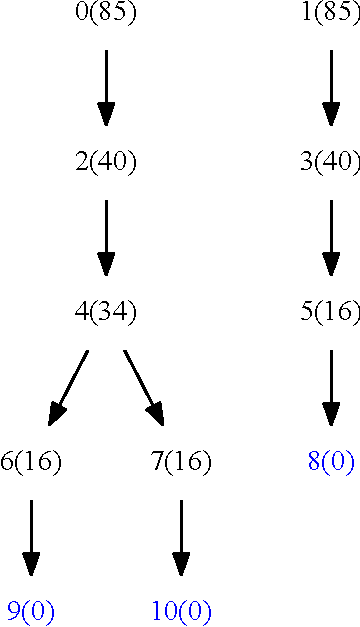
\includegraphics[width=.28\textwidth]{../paper/fig/1S1L-ext.pdf}
}
\end{figure}
\end{frame}

\begin{frame}
\begin{figure}
\centering
\setcounter{subfigure}{0}
\subfigure[]{
    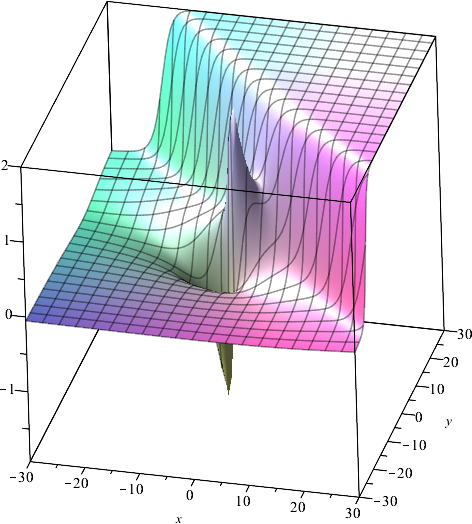
\includegraphics[width=.3\textwidth]{../paper/fig/1S1L-1.png}
}
\subfigure[]{
    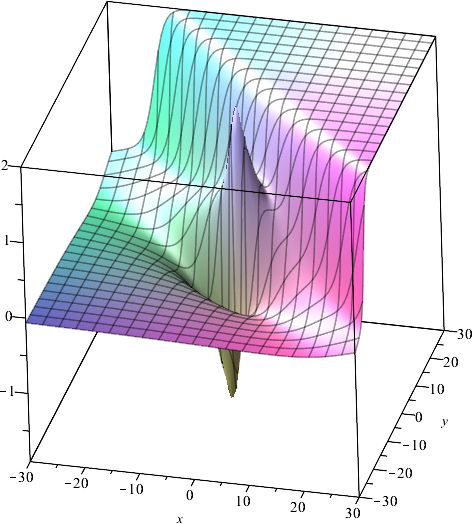
\includegraphics[width=.3\textwidth]{../paper/fig/1S1L-2.png}
}
\subfigure[]{
    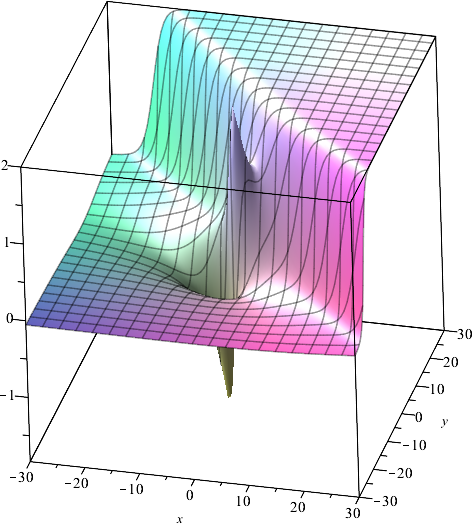
\includegraphics[width=.3\textwidth]{../paper/fig/1S1L-3.png}
}
\caption{(3+1)维 YTSF 方程的 1S-1L 解} \label{fig-1S1L}
\end{figure}
\end{frame}

\frame{
\begin{figure}
\centering
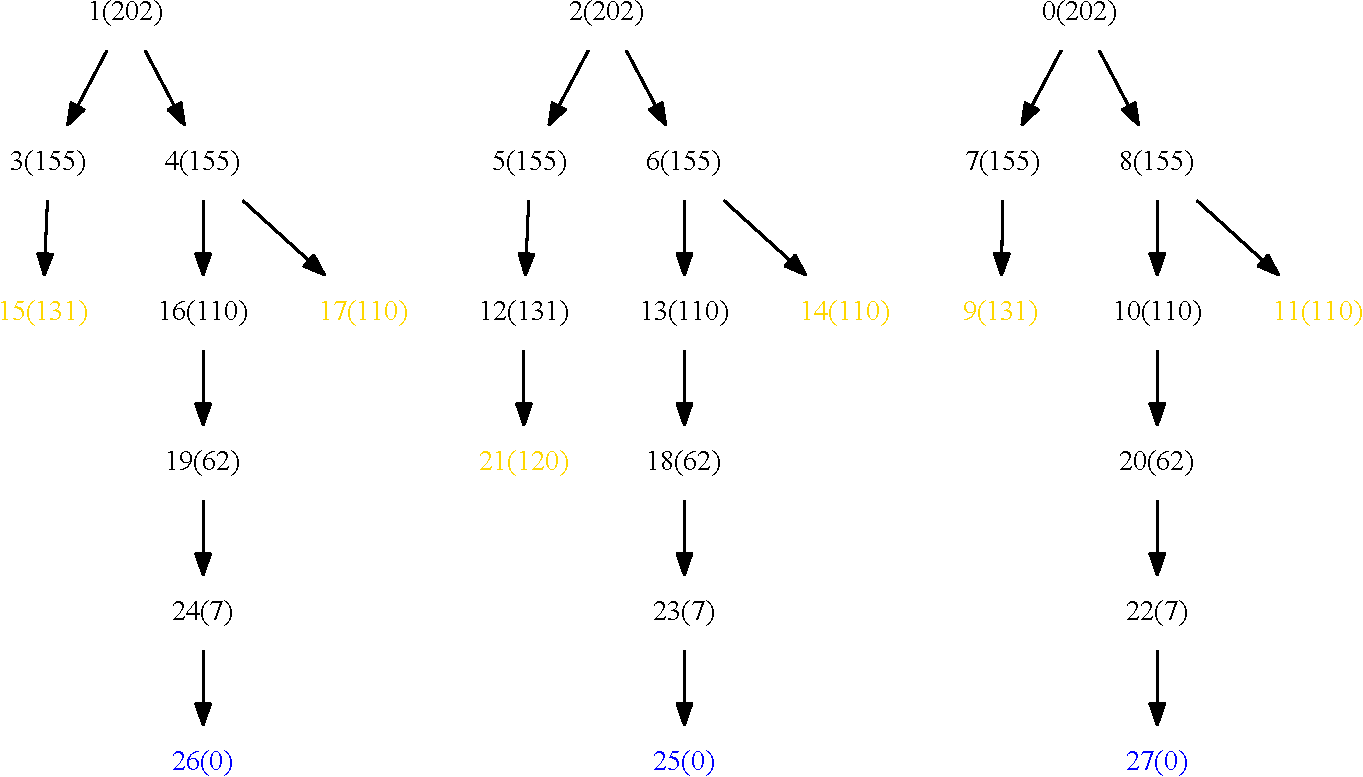
\includegraphics[width=\textwidth]{../paper/fig/2S1L-ext.pdf}
\caption{2S-1L 继承求解的分支图(30 秒)}\label{sb2-e}
\end{figure}
}

\begin{frame}
\begin{figure}
\centering
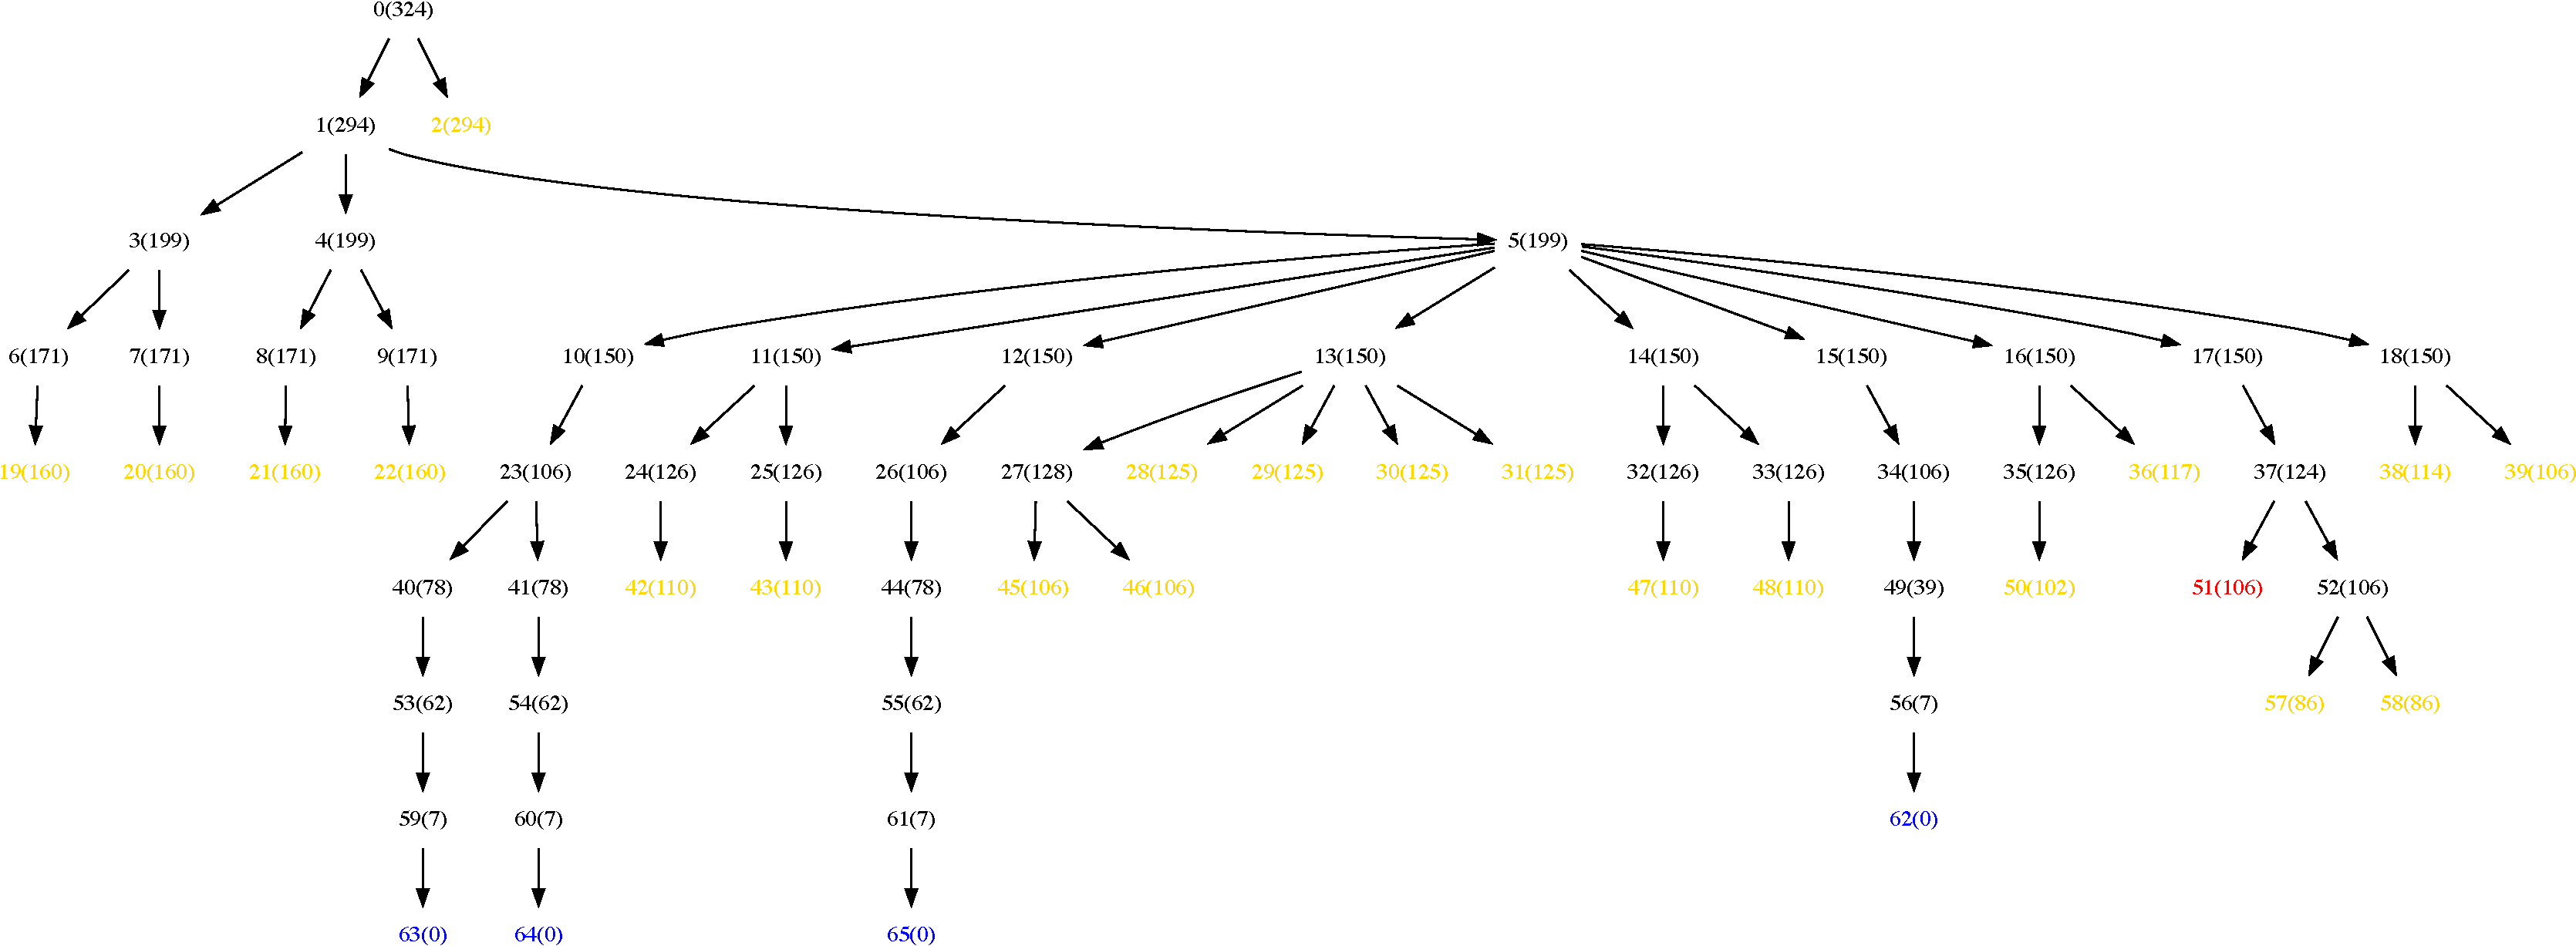
\includegraphics[width=\textwidth]{2S1L-dir-number.pdf}
\caption{2S-1L 直接求解的分支图(430 秒)}\label{sb2-d-n}
\end{figure}
\end{frame}

\frame{
\begin{figure}
\centering
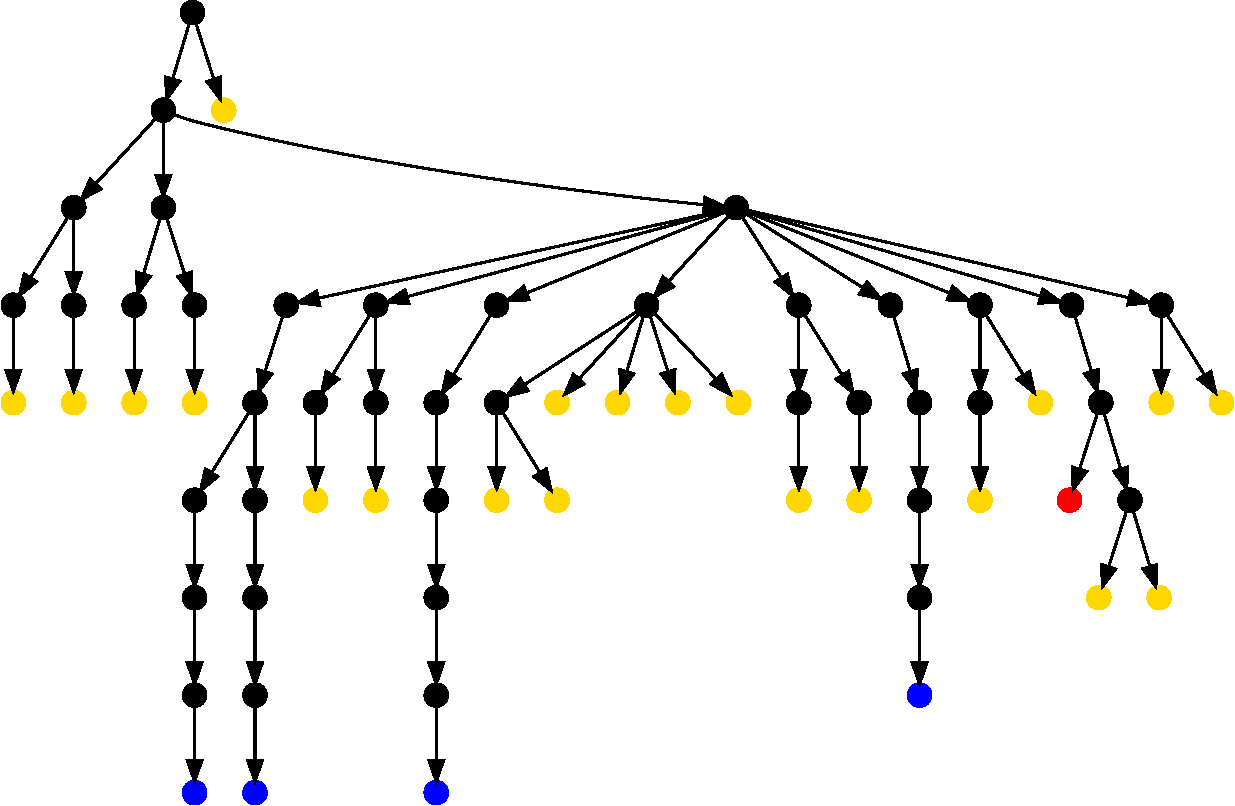
\includegraphics[height=0.8\textheight]{2S1L-dir-point.pdf}
\caption{2S-1L 直接求解的分支图(430 秒)}\label{sb2-d-p}
\end{figure}
}

\frame{
\begin{figure}
\centering
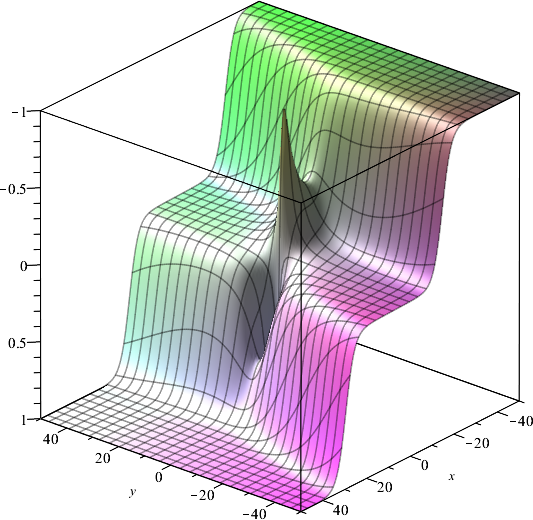
\includegraphics[width=.6\textwidth]{../paper/fig/2S1L.png}
\caption{(3+1)维 YTSF 方程的 2S-1L 解} \label{fig-2S1L}
\end{figure}
}

\begin{frame}
\frametitle{求解效率对比}
\begin{adjustbox}{max width=\textwidth}
\centering
\renewcommand{\arraystretch}{1.3}
\begin{tabular}{cccccc}
\hline
来源方程 & 阶数 & 方程数 & 变量数 & PGSolve用时 & Solve用时 \\
\hline
(2+1) SK & 0 & 20 & 9 & 0.724 & 3.483 \\
(2+1) BKP-T & 0 & 20 & 9 & 0.571 & 3.486 \\
(2+1) KP & 0 & 35 & 9 & 1.759 & 29.643 \\
(3+1) YTSF & 0 & 35 & 11 & 1.229 & 8.839 \\
(3+1) JM & 0 & 35 & 11 & 0.845 & >1800 \\
(2+1) SK & 1 & 65 & 13 & 10.241 & >1800 \\
(3+1) YTSF & 1 & 120 & 16 & 12.228 & 1696.852 \\
\hline
\end{tabular}
\end{adjustbox}

\vspace{1em}

此处对比的是\cd{PDEtools:-Solve}. 而最常用的\cd{solve}函数甚至不能在 72 小时内求解只有 20 个方程的方程组, 这显然是\cd{solve}函数的一个 BUG.

\end{frame}

\begin{frame}

\begin{adjustbox}{max width=\textwidth}
\renewcommand{\arraystretch}{1.3}
\begin{tabular}{cccccc}
\hline
方程名称    & 解的阶数 & 方程数量 & 分组大小 & 解的个数 & 运行时间(s) \\ 
\hline 
(2+1)SK & 0 & 20 & 5 & 1 & 2.197 \\
(2+1)SK & 1 & 65 & 3 & 1 & 3.072 \\
(2+1)SK & 2 & 179 & 5 & 2 & 12.697 \\
(2+1)BKP-T & 0 & 20 & 5 & 1 & 1.036 \\
(2+1)BKP-T & 1 & 65 & 3 & 1 & 3.251 \\
(2+1)BKP-T & 2 & 179 & 5 & 2 & 12.617 \\
(3+1)YTSF & 0 & 35 & 5 & 2 & 1.948 \\
(3+1)YTSF & 1 & 120 & 5 & 3 & 6.717 \\
(3+1)YTSF & 2 & 324 & 5 & 3 & 37.909 \\
(3+1)JM & 0 & 35 & 5 & 3 & 2.014 \\
(3+1)JM & 1 & 120 & 5 & 13 & 18.384 \\
(3+1)JM & 2 & 324 & 5 & 4 & 50.934 \\
\hline 
\end{tabular}
\end{adjustbox}
\end{frame}

\begin{frame}
我们还通过推广简单Hirota方法构造不同的相互作用解.
\begin{figure}
\subfigure[2-孤子,1-呼吸子,1-lump]{
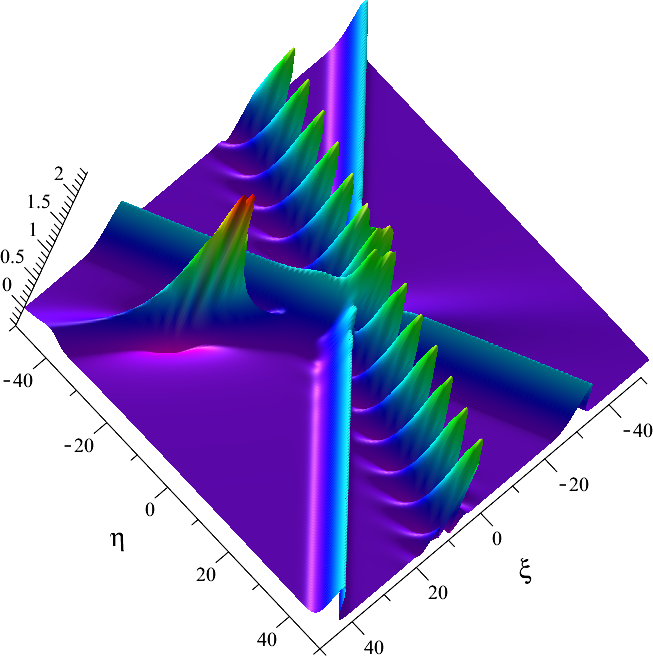
\includegraphics[width=.45\textwidth]{(4+1)Fokas-112.png}
}
\subfigure[1-孤子,2-呼吸子,2-lump]{
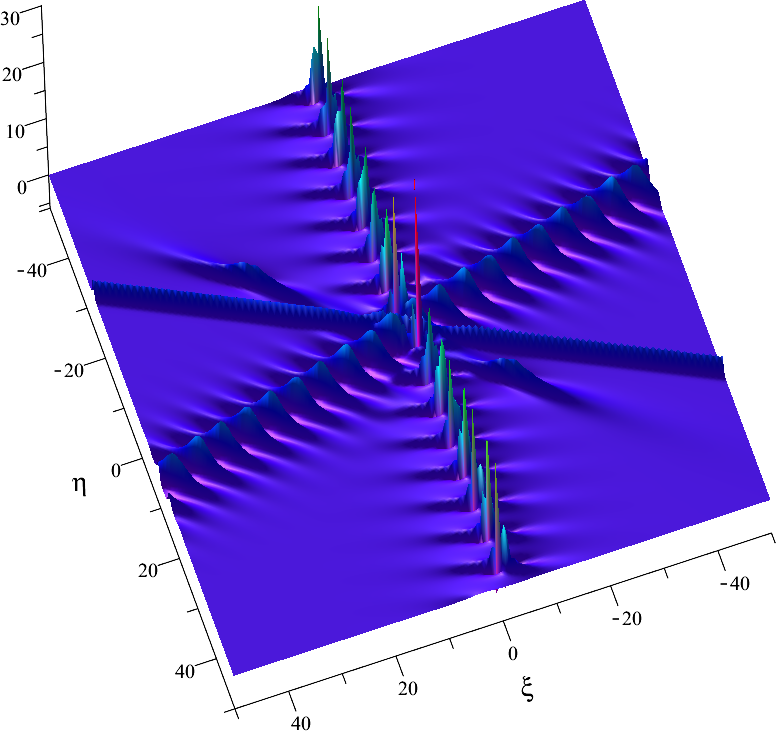
\includegraphics[width=.45\textwidth]{(4+1)Fokas-221.png}
}
\caption{(4+1)Fokas 方程的高阶相互作用解}
\end{figure}
\end{frame}

\section{致谢}
\begin{frame}
\tikz[overlay,remember picture]\node[opacity=0.2]at (current page.center){
\includegraphics[width=0.7\paperheight]{../paper/sty/ecnu_logo.pdf}};
\centerline{\Huge 谢谢}
\end{frame}
\end{document}